\documentclass[
	% -- opções da classe memoir --
	12pt,				% tamanho da fonte
	openright,			% capítulos começam em pág ímpar (insere página vazia caso preciso)
	twoside,			% para impressão em recto e verso. Oposto a oneside
	a4paper,			% tamanho do papel. 
	% -- opções da classe abntex2 --
	chapter=TITLE,		% títulos de capítulos convertidos em letras maiúsculas
	%section=TITLE,		% títulos de seções convertidos em letras maiúsculas
	%subsection=TITLE,	% títulos de subseções convertidos em letras maiúsculas
	%subsubsection=TITLE,% títulos de subsubseções convertidos em letras maiúsculas
	% -- opções do pacote babel --
	english,			% idioma adicional para hifenização
	french,				% idioma adicional para hifenização
	spanish,			% idioma adicional para hifenização
	brazil				% o último idioma é o principal do documento
	]{abntex2}

%Importa todos os pacotes básicos para a estruturação do projeto

% ---
% Pacotes básicos 
% ---
\usepackage{lmodern}			% Usa a fonte Latin Modern			
\usepackage[T1]{fontenc}		% Selecao de codigos de fonte.
\usepackage[utf8]{inputenc}		% Codificacao do documento (conversão automática dos acentos)
%\usepackage{indentfirst}		% Indenta o primeiro parágrafo de cada seção.
\usepackage{color}				% Controle das cores
\usepackage{graphicx}			% Inclusão de gráficos
\usepackage{microtype} 			% para melhorias de justificação
\usepackage{multicol}
\usepackage{color}
\usepackage{layouts}
%\usepackage{float}

\usepackage[dvipsnames*,svgnames]{xcolor}
\usepackage[most]{tcolorbox}

\usepackage{doctum}
% ---

\usepackage[scaled]{helvet}
\renewcommand*\familydefault{\sfdefault}		
% ---
% Pacotes adicionais, usados apenas no âmbito do Modelo Canônico do abnteX2
% ---
\usepackage{lipsum}				% para geração de dummy text
% ---

% ---
% Pacotes de citações
% ---
\usepackage[brazilian,hyperpageref]{backref}	 % Paginas com as citações na bibl
\usepackage[abnt-emphasize=bf,alf]{abntex2cite}	% Título da citação em negrito

% --- 
% CONFIGURAÇÕES DE PACOTES
% --- 
\setlrmarginsandblock{3cm}{2cm}{*}
\setulmarginsandblock{3cm}{2cm}{*}
\checkandfixthelayout

% ---
% Configurações do pacote backref
% Usado sem a opção hyperpageref de backref
\renewcommand{\backrefpagesname}{Citado na(s) página(s):~}
% Texto padrão antes do número das páginas
\renewcommand{\backref}{}
% Define os textos da citação
\renewcommand*{\backrefalt}[4]{
	\ifcase #1 %
		Nenhuma citação no texto.%
	\or
		Citado na página #2.%
	\else
		Citado #1 vezes nas páginas #2.%
	\fi}%
% ---

%-------------------------------------------------

% ---
% Informações de dados para CAPA e FOLHA DE ROSTO
% ---
\titulo{Visão computacional aplicada no reconhecimento de jogadores de futebol americano}

\autor{THAYRONE MARQUES SILVA
 \\	VINÍCIUS ANDRADE LOPES}
 
\local{IPATINGA, MG}

\data{2019}

\orientador{Esp. Tales Wallace Souza}
% \coorientador{Equipe \abnTeX}
\instituicao{%
  FACULDADES DOCTUM DE IPATINGA
  \par
  BACHARELADO EM SISTEMAS DE INFORMAÇÃO}
\tipotrabalho{Trabalho de Conclusão de Curso}
% O preambulo deve conter o tipo do trabalho, o objetivo, 
% o nome da instituição e a área de concentração 
\preambulo{Este Trabalho de Conclusão de Curso foi julgado e aprovado, como requisito parcial a obtenção do título de bacharel em Sistemas de Informação na Faculdade Doctum de Ipatinga – Rede Doctum de Ensino, em 2018.}
% ---


% ---
% Configurações de aparência do PDF final

% alterando o aspecto da cor azul
\definecolor{blue}{RGB}{41,5,195}

% informações do PDF
\makeatletter
\hypersetup{
     	%pagebackref=true,
		pdftitle={\@title}, 
		pdfauthor={\@author},
    	pdfsubject={\imprimirpreambulo},
	    pdfcreator={LaTeX with abnTeX2},
		pdfkeywords={abnt}{latex}{abntex}{abntex2}{trabalho acadêmico}, 
		colorlinks=true,       		% false: boxed links; true: colored links
    	linkcolor=blue,          	% color of internal links
    	citecolor=blue,        		% color of links to bibliography
    	filecolor=magenta,      		% color of file links
		urlcolor=blue,
		bookmarksdepth=4
}
\makeatother
% --- 

% ---
% Posiciona figuras e tabelas no topo da página quando adicionadas sozinhas
% em um página em branco. Ver https://github.com/abntex/abntex2/issues/170
\makeatletter
\setlength{\@fptop}{5pt} % Set distance from top of page to first float
\makeatother
% ---

% ---
% Possibilita criação de Quadros e Lista de quadros.
% Ver https://github.com/abntex/abntex2/issues/176
%
\newcommand{\quadroname}{Quadro}
\newcommand{\listofquadrosname}{Lista de quadros}

\newfloat[chapter]{quadro}{loq}{\quadroname}
\newlistof{listofquadros}{loq}{\listofquadrosname}
\newlistentry{quadro}{loq}{0}

% configurações para atender às regras da ABNT
\setfloatadjustment{quadro}{\centering}
\counterwithout{quadro}{chapter}
\renewcommand{\cftquadroname}{\quadroname\space} 
\renewcommand*{\cftquadroaftersnum}{\hfill--\hfill}

\setfloatlocations{quadro}{hbtp} % Ver https://github.com/abntex/abntex2/issues/176
% ---

% --- 
% Espaçamentos entre linhas e parágrafos 
% --- 

% O tamanho do parágrafo é dado por:
\setlength{\parindent}{0cm}

% Controle do espaçamento entre um parágrafo e outro:
%\setlength{\parskip}{1.5em}  % tente também \onelineskip

\setlength{\parskip}{1.5em}

%\setlength\afterchapskip{1.5em}

% ---
% Compila o indice
% ---
\makeindex
% ---


% ----
% Início do documento
% ----
\begin{document}
% Seleciona o idioma do documento (conforme pacotes do babel)
%\selectlanguage{english}
\selectlanguage{brazil}

% Retira espaço extra obsoleto entre as frases.
\frenchspacing 

% ----------------------------------------------------------
% ELEMENTOS PRÉ-TEXTUAIS
% ----------------------------------------------------------
% \pretextual

% ---
% Capa
% ---
\imprimircapa
% ---

% ---
% Folha de rosto
% (o * indica que haverá a ficha bibliográfica)
% ---
\imprimirfolhaderosto*
% ---

% ---
% Inserir a ficha bibliografica
% ---

% Isto é um exemplo de Ficha Catalográfica, ou ``Dados internacionais de
% catalogação-na-publicação''. Você pode utilizar este modelo como referência. 
% Porém, provavelmente a biblioteca da sua universidade lhe fornecerá um PDF
% com a ficha catalográfica definitiva após a defesa do trabalho. Quando estiver
% com o documento, salve-o como PDF no diretório do seu projeto e substitua todo
% o conteúdo de implementação deste arquivo pelo comando abaixo:

\begin{fichacatalografica}
	\sffamily
	\vspace*{\fill}					% Posição vertical
	\begin{center}					% Minipage Centralizado
	\fbox{\begin{minipage}[c][8cm]{13.5cm}		% Largura
	\small
	\imprimirautor
	%Sobrenome, Nome do autor
	
	\hspace{0.5cm} \imprimirtitulo  / \imprimirautor. --
	\imprimirlocal, \imprimirdata-
	
	\hspace{0.5cm} \thelastpage p. : il. (algumas color.) ; 30 cm.\\
	
	\hspace{0.5cm} \imprimirorientadorRotulo~\imprimirorientador\\
	
	\hspace{0.5cm}
	\parbox[t]{\textwidth}{\imprimirtipotrabalho~--~\imprimirinstituicao,
	\imprimirdata.}\\
	
	\hspace{0.5cm}
		1. Visão Computacional.
		2. Processamento de Imagem.
		3. Reconhecimento.
		I. Esp. Tales Wallace Souza.
		II. Faculdades DOCTUM de Ipatinga.
		III. \imprimirtipotrabalho 			
	\end{minipage}}
	\end{center}
\end{fichacatalografica}
% ---

% ---
% Inserir folha de aprovação
% ---

% Isto é um exemplo de Folha de aprovação, elemento obrigatório da NBR
% 14724/2011 (seção 4.2.1.3). Você pode utilizar este modelo até a aprovação
% do trabalho. Após isso, substitua todo o conteúdo deste arquivo por uma
% imagem da página assinada pela banca com o comando abaixo:
%
% \begin{folhadeaprovacao}
% \includepdf{folhadeaprovacao_final.pdf}
% \end{folhadeaprovacao}
%
\setlength{\ABNTEXsignwidth}{12cm}
\begin{folhadeaprovacao}

  \begin{center}
    {\ABNTEXchapterfont\large\imprimirautor}

    \vspace*{\fill}\vspace*{\fill}
    \begin{center}
      \ABNTEXchapterfont\bfseries\Large\imprimirtitulo
    \end{center}
    \vspace*{\fill}
    
    \hspace{.45\textwidth}
    \begin{minipage}{.5\textwidth}
        \imprimirpreambulo
        
        \vspace{1cm}
        
        Média Final: \rule{3cm}{0.2mm}
    \end{minipage}%
    \vspace*{\fill}
   \end{center}
        
   Ipatinga, XX de dezembro de 20XX
   
   \vspace{1cm}
   
   \centering\textbf{Banca Examinadora}

   \assinatura{Prof. Orientador: \imprimirorientador \\ MBA em Gerenciamento de Projetos Doctum \\ Instituto Superior Doctum de Ipatinga
   } 
   \assinatura{Prof.ª Convidada: Maíza Cristina de Souza Dias \\ Mestre em Informática PUC-Minas \\ Instituto Superior Doctum de Ipatinga}
   \assinatura{Prof. Convidado: Giovani Scarabelli Silva \\ Especialista em Administração de Sistema de Informação - UFLA \\ Instituto Superior Doctum de Ipatinga}
   %\assinatura{\textbf{Professor} \\ Convidado 3}
   %\assinatura{\textbf{Professor} \\ Convidado 4} 
\end{folhadeaprovacao}
% ---

% ---
% Dedicatória
% ---
\begin{dedicatoria}[DEDICATÓRIA]
Dedico este trabalho primeiramente a Deus que nos sustentou durante toda a jornada. A nossos familiares e entes queridos, que acreditaram desde o início em nós.
\end{dedicatoria}
% ---

% ---
% Agradecimentos
% ---
\begin{agradecimentos}[AGRADECIMENTOS]
Agradecemos primeiramente a Deus que esteve conosco em todas as tribulações de nossas vidas, nos ajudando a superá-las.

Aos nossos pais, por todo o amor que nos deram, além da educação, ensinamentos e apoio. A nossos entes queridos que estiveram conosco durante toda esta caminhada.

A todo o corpo docente das Faculdades Doctum de Ipatinga que esteve presente em todos os momentos de nossos estudos, em especial para o nosso professor orientador Tales Wallace Souza, que nos auxiliou com todo seu profissionalismo para o desenvolvimento deste trabalho e a Maíza Cristina de Souza Dias, que contribuiu com seu conhecimento e especialidade sobre o assunto decorrente deste trabalho.

E finalmente, mas não menos importante, a todos os integrantes da turma de sistemas de informação, que percorreram toda esta jornada conosco.
\end{agradecimentos}
% ---

% ---
% Epígrafe
% ---
\begin{epigrafe}
\vspace*{\fill}
\begin{flushright}
\textit{Quando todos nos unirmos contra as \\
injustiças e em defesa da privacidade e \\
dos direitos humanos básicos, poderemos nos \\
defender até dos mais poderosos dos sistemas. \\}
\vspace{3mm}
(\textit{Edward Snowden})
\end{flushright}
\end{epigrafe}
% ---

% ---
% RESUMOS
% ---

% resumo em português
\setlength{\absparsep}{18pt} % ajusta o espaçamento dos parágrafos do resumo
%resumo em português
\begin{resumo}[RESUMO]
A visão computacional vem sendo utilizada em larga escala, sendo difundida em várias áreas no mercado atual. Indústria e áreas desportivas são exemplos de áreas que têm apresentado um crescimento expressivo devido as soluções empregadas pela tecnologia citada. No entanto, a implantação deste tipo de tecnologia requer um conhecimento avançado sobre esta e também sobre as regras de negócios que serão aplicadas para a resolução de algum problema em específico. Como consequência disto, o investimento em \textot{hardwares} que são capazes de realizar altos níveis de processamento também deve ser levando em consideração, visto que um computador básico não tem potência suficiente para realizar análises de imagem em tempo real. Sendo assim, esta pesquisa exploratória tem a finalidade de apresentar, de maneira didática, o funcionamento da tecnologia de visão computacional aplicada no esporte futebol americano onde, a princípio, foi proposto o reconhecimento de um dos jogadores dentro de campo.

 \textbf{Palavras-chave}: Visão computacional. Processamento de imagem. Reconhecimento. Tecnologia.
\end{resumo}

% resumo em inglês
\begin{resumo}[ABSTRACT]
 \begin{otherlanguage*}{english}
Computer vision has been used on a large scale and is widespread in many areas of the current market. Industry and sports are examples of areas that have shown significant growth due to the solutions employed by the technology mentioned. However, deploying this type of technology requires advanced knowledge of this technology as well as the business rules that will be applied to solve any particular problem. As a consequence of this, the investment in hardware that is capable of performing high processing levels must also be taken into consideration, as a basic computer does not have enough power to perform real-time image analysis. Thus, this exploratory research has the purpose of presenting, in a didactic way, the operation of computer vision technology applied in the football sport where, at first, the recognition of one of the players on the field was proposed.

   \noindent 
   \textbf{Keywords}: Computer Vision. Image Processing. Recognition. Technology.
 \end{otherlanguage*}
\end{resumo}
% ---

% ---
% inserir lista de ilustrações
% ---
\pdfbookmark[0]{\listfigurename}{lof}
\listoffigures*
\cleardoublepage
% ---

% ---
% inserir lista de quadros
% ---
\pdfbookmark[0]{\listofquadrosname}{loq}
\listofquadros*
\cleardoublepage
% ---

% ---
% inserir lista de tabelas
% ---
\pdfbookmark[0]{\listtablename}{lot}
\listoftables*
\cleardoublepage
% ---

% ---
% inserir lista de abreviaturas e siglas
% ---
\begin{siglas}
  \item[2-D] Duas dimensões
  \item[API] \textit{Application Programming Interface}
  \item[APS] \textit{Active Pixel Sensor}
  \item[BSD] \textit{Berkeley Software Distribution}
  \item[CCD] \textit{Charge Coupled Devic}
  \item[CIE] Comissão Internacional de Iluminação
  \item[CMOS] \textit{Complementary Metal Oxide Semiconducto}
  \item[IDE] \textit{Integrated Development Environment}
  \item[MOS] \textit{Metal Oxide Semiconductor}
  \item[NASA] \textit{National Aeronautics and Space Administration}
  \item[NFL] \textit{National Football League}
  \item[OpenCV] \textit{Open Source Computer Vision Library}
  \item[RCS] \textit{Revision Control System}
  \item[RGB] \textit{Red (Vermelho), Green (Verde) e Blue (Azul)}
  \item[SCM] \textit{Source Code Manager}
  \item[VCS] \textit{Version Control System}
\end{siglas}
% ---

% ---
% inserir lista de símbolos
% ---
%\begin{simbolos}
  \item[$ \Gamma $] Letra grega Gama
  \item[$ \Lambda $] Lambda
  \item[$ \zeta $] Letra grega minúscula zeta
  \item[$ \in $] Pertence
\end{simbolos}
% ---

% ---
% inserir o sumario
% ---
\pdfbookmark[0]{\contentsname}{toc}
\tableofcontents*
\cleardoublepage
% ---



% ----------------------------------------------------------
% ELEMENTOS TEXTUAIS
% ----------------------------------------------------------
\textual

\pagestyle{simple}

\chapter{\textbf{INTRODUÇÃO}}
\label{cap-introducao}
A evolução tecnológica expandiu consideravelmente nos dias atuais, proporcionando um avanço descomunal de vários \textit{hardwares} poderosíssimos capazes de realizar tarefas jamais vistas pelos gênios antigos da computação. Devido a isso, imersões de várias técnicas vêm sendo estudadas progressivamente nos últimos anos, visto que atualmente existem equipamentos capazes de realizá-las em um curto prazo de tempo e de maneira mais eficaz.

A área de visão computacional se tornou de grande interesse nos tempos atuais devido à sua complexidade ao realizar processamentos de imagens e extrair o maior número de informações desta. O campo de processamento de imagem complementa esta parte, utilizando técnicas matemáticas e probabilísticas para corrigir os parâmetros visuais da imagem que será processada.

Por mais que existam alguns problemas nesta área como, por exemplo, a captura de imagens, processamento, alta precisão, similaridade, dentre outros, os estudos buscam aprimorar a ferramenta para que o campo de visão computacional se aproxime ou até ultrapasse, em algumas situações, à eficiência da uma visão humana.

O futebol americano é um esporte bastante popular nos Estados Unidos da América (EUA), na frente até mesmo de grandes esportes como, por exemplo, \textit{baseball}, \textit{basketball} e \textit{football}. Em 1869, nos EUA, aconteceu o primeiro jogo de futebol americano no mundo, onde a Universidade de \textit{Princeton} recebia o time da Universidade de \textit{Rugters}. Na época, o futebol americano ainda estava tomando forma, sem muitas regras e muito confuso. Mesmo assim, o esporte se popularizou, principalmente dentre os universitários \cite{RODRIGUES2014}. No Brasil o esporte tem se popularizado nos últimos anos devido ao fato das redes de TV por assinatura transmitirem o evento em larga escala (\autoref{mercado-do-futebol-americano}). 

\section{\textbf{{Objetivo geral}}}
\label{objetivo-geral}
Apresentar uma ferramenta que seja capaz de identificar um jogador de futebol americano dentro de campo. Para isso, a identificação será feita através de uma ferramenta a ser desenvolvida utilizando visão computacional e a biblioteca de processamento de imagens \textit{OpenCV}. 


\section{\textbf{{Objetivos específicos}}}
 \begin{itemize}
\item Classificar as imagens de um jogador de futebol americano e extrair o maior numero de informações;

\item Treinar o algoritmo seguindo as informações classificadas;

\item Elaborar um modelo de busca com o conjunto de informações processadas sobre jogadores de futebol americano;
   
\item Capturar, através de um dispositivo de entrada de vídeo, as imagens de uma partidade futebol americano;
   
\item Identificar o jogador seguindo o modelo de busca;
   
\item Analisar o percentual de acertos e erros da ferramenta.
   
 \end{itemize}
\section{\textbf{Justificativa}}

A área de visão computacional tem crescido de forma significativa no mundo presente, devido ao avanço tecnológico. Várias informações são capturadas e o volume de dados encontram-se crescendo progressivamente. Sendo assim, inumeras aplicações que utilizam a tecnologia de visão computacional estão sendo desenvolvidas para auxiliar diversas áreas, como por exemplo a medicina, segurança e esporte.

Este crescimento ocorre principalmente devido ao aumento da utilização de dispositivos móveis. Não é difícil se deparar com vários equipamentos que já utilizam essa tecnologia para alguma função, seja ela para melhorar algo, seja para realizar a identificação de algum objeto ou biometria de segurança, como por exemplo o \textit{Face ID} (Identidade de Rosto) da \textit{Apple} e o \textit{Google Lens}.

Sendo assim, a visão computacional pode auxiliar na questão relacionada ao reconhecimento de um jogador em uma partida de futebol americano.

As jogadas realizadas em futebol americano são de total contato físico e de alta velocidade. As transições dos jogadores são feitas em vários momentos para que as jogadas certas possam acontecer de acordo com a tática traçada pelo técnico. A leitura dessas substituições rápidas são feitas a olho humano, onde podem ocorrer equívocos e possíveis erros na identificação dos jogadores.

Outro fator crucial é que o mercado de futebol americano é muito valioso. Conforme descrito com mais detalhes na \autoref{mercado-do-futebol-americano} deste projeto, a \textit{NFL - National Football League} (Liga Nacional de Futebol) é a liga desportiva mais rica do mundo. A revista \citeonline{FORBES2019} descreve que a liga investe grandemente em ferramentas de \textit{marketing} digital e tecnologias que auxiliam no desempenho dos jogos. Dan Lovinger, vice-presidente executivo de vendas de publicidade da rede de transmissão \textit{NBC Sports}, informa que o preço médio de um comercial de 30 segundo no ar gira em torno de U\$ 5 milhões, totalizando um gasto médio de aproximadamente U\$ 500 milhões durante apenas uma partida de futebol americano. O show do intervalo patrocinado pela empresa \textit{Pepsi} mantêm um acordo que custa cerca de U\$ 7 milhões por ano, segundo o \textit{Sports Business Journal}. O valor dos ingressos do \textit{Super Bowl} varia entre U\$ 950 e U\$ 5 mil (Assentos \textit{Premium}), onde esses valores podem alcançar níveis mais altos em mercados paralelos. Outro fator que esta em grande crescimento dentre a população que acompanha a \textit{NFL} é o numero de apostas no evento \textit{Super Bowl}, que é denominado o melhor evento para realizar apostas. Na 51\textsuperscript{\underline{a}} edição do evento, o \textit{Nevada Gaming Control Board} (Conselho de Controle de Jogos de Nevada) registrou um recorde de U\$ 138,5 milhões em apostas \cite{FORBES2018}.

Com base nisso, pode-se reconhecer a importância de realizar um tratamento minucioso nos dados das partidas, para que não ocorra nenhum equívoco dentro de campo que pode comprometer algum índice.
\section{\textbf{Organização do trabalho}}

Este trabalho é composto por cinco capítulos, estruturados da seguinte forma: o \autoref{cap-fundamentos-conceituais} é composto pelos fundamentos conceituais que foram necessários para o entendimento da área de visão computacional. No \autoref{metodologia} foi abordada a metodologia utilizada para a construção deste trabalho.  Subsequente, o \autoref{desenvolvimento} relata todo o desenvolvimento do trabalho, ressaltando todas as etapas de funcionamento, descrição do sistema,  restrições, riscos e exclusões do projeto, requisitos funcionais e não-funcionais, explicação do código, etapa de testes e análise do \textit{software} e avaliação dos resultados. Por fim, o \autoref{consideracoes_finais} apresenta as considerações finais obtidas com o projeto, seguida das propostas de novos estudos.

% ----------------------------------------------------------
% PARTE
% ----------------------------------------------------------
%TODO TWS REMOVER PART \part{Preparação da pesquisa}
% ----------------------------------------------------------

%-- Inicio conteúdo bibliográficoo --%

\chapter{\textbf{FUNDAMENTOS CONCEITUAIS}}
\label{cap-fundamentos-conceituais}

Este capitulo tem por objetivo descrever o referencial teórico usado para a elaboração deste trabalho cientifico e suas fundamentações. O capitulo está dividido em seções que abordam os principais temas utilizados no desenvolvimento do contexto bibliográfico. A \autoref{futebol-americano} relata o contexto de futebol americano e tecnologias aplicadas no meio desportivo. Ja a \autoref{visao-computacional} descreve os conceitos de visão computacional e as etapas do processamento de imagem, exemplificando as principais tecnologias utilizadas neste contexto. A \autoref{engenharia-software} trata os conceitos de Engenharia de \textit{Software} e suas metodologias ágeis. Para finalizar, a \autoref{ferramentas-de-desenvolvimento-do-projeto} descreve todas as ferramentas fundamentais para o desenvolvimento desse projeto.

\section{\textbf{{Futebol Americano}}}
\label{futebol-americano}

O futebol americano é um esporte que se destaca devido ao porte físico de seus atletas e as disputas de força dentro de campo. O tempo de duração de uma partida pode demorar várias horas dependendo das pontuações em questão.

Do mesmo modo, vários jogadores participam de inúmeras jogadas dentro de campo, e é muito complexo acompanhar todas elas de forma detalhada, até mesmo para as pessoas que são treinadas e capacitadas para as analisarem.

O futebol americano consiste de uma série de jogadas, objetivando alcançar jardas\footnote{Jarda é um termo muito utilizado em países anglo-americanos que representam distâncias curtas. No futebol americano, as distâncias percorridas pelos jogadores são representadas por jardas. Cada jarda corresponde a aproximadamente 0,91 metros \cite{BRASILESCOLA2019}.\label{Jardas}} para somar mais pontos que seu adversário. Cada jogada consiste em 4 tentativas de avançar mais jardas do campo adversário. São 22 jogadores dentro de campo com possibilidades infinitas de substituição enquanto a bola não estiver em jogo. Um time tenta avançar e outro tenta impedir esse avanço: caso o time atacante consiga as jardas, ele continua com a posse de bola; caso contrário, o time adversário recebe a bola de volta e inicia a sua tentativa de ganhar jardas e chegar a \textit{End Zone} (Zona Final) \cite{NFL2019}.

Sua origem, datada em 1876, teve suas regras e seu modo de jogo evoluídas até chegar a um ponto onde a tecnologia pareava com o esporte, proporcionando uma velocidade acima da média nos resultados e na competitividade entre os jogadores da modalidade. Os treinadores começaram a utilizar alguns recursos para conseguir os melhores resultados dentro e fora de campo. Assim, a tecnologia se tornou um dos pilares de um time de ponta ao longo das competições. Sabe-se que o esporte é algo totalmente imprevisível mas existem pessoas que discordam dessa afirmação. De acordo com \citeonline{NEPOMUCENO2012}, todos os times que utilizam estatísticas e análise de dados têm vantagens sobre os seus adversários.

Atualmente, os dados obtidos manualmente por times e técnicos são coletados e em seguida, analisados por ferramentas de estatística. Dessa forma, se torna mais simples reconhecer os padrões e entregar informações que não são obtidas usando apenas a capacidade cognitiva e intelectual humana.

Com um número enorme de jogadores para avaliar durante a temporada do futebol profissional, o melhor modo para que treinadores, dirigentes e olheiros das equipes possam ter melhores hipóteses de quais jogadores possuem o potencial para agregar um melhor desempenho ao time, é agrupar candidatos em um lugar onde todos pudessem mostrar suas habilidades. O \textit{Draft} é um evento anual onde os times grandes podem analisar e selecionar jogadores de futebol americano universitário para reforçar o seu elenco. Esse é um dos maiores eventos que acontece na intertemporada da \textit{NFL}. Já o \textit{Combine} é um evento que acontece antes do \textit{Draft}, que proporciona aos executivos, técnicos e responsáveis pelo departamento pessoal, realizarem uma análise da capacidade física e mental dos jogadores universitários \cite{MCGEE2003}.

Sendo assim, ter dados precisos sobre as habilidades destes jogadores e compará-las com outros jogadores participantes do \textit{Combine} e do próprio elenco também é útil para auxílio nas estratégias e no posicionamento de cada atleta selecionado.

De acordo com \citeonline{BASS2012} um exemplo claro disto é a avaliação dos \textit{quarterbacks}. Com a grande necessidade dos times por um jogador que lidere os ataques, observar bem os jogadores da posição durante o \textit{Combine} pode ser decisivo no momento em que um time define se vale a pena escolher um \textit{quarterback} no \textit{Draft} (Evento que acontece depois do \textit{Combine}), manter um que já está no elenco ou partir para o mercado em busca do substituto que possa cumprir com as expectativas da equipe.

Para os jogadores, o \textit{Combine} é a melhor forma de tentar impressionar os observadores das equipes e convencê-los de que ele pode ser o atleta ideal. Quem se destaca com bons números durante os testes pode ver sua cotação aumentar nas listas das equipes e até ter a chance de ser escolhido durante a primeira rodada do \textit{Draft}, uma oportunidade que apenas 32 jogadores conseguem a cada ano.

\subsection{Tecnologias aplicadas no esporte}

O contexto da tecnologia atual vem sendo aplicado a passos largos na área desportiva. Tal ação proporciona uma enorme mudança nos resultados, gerando discussões relacionadas ao benefício e malefício desse progresso.

\citeonline{KATZ1989} explicam que com o uso de técnicas do meio desportivo incorporadas a tecnologia, é possível ampliar a performance e a inteligência dos atletas, fazendo com que as habilidades dos atletas seja cada vez mais aprimorada.

Isso ocorre porque atualmente os atletas possuem um grande número de tecnologias para os auxiliarem no esporte. Vários \textit{softwares} e ferramentas auxiliam os profissionais a estarem sempre preparados fisicamente e psicologicamente para exercer a sua tarefa.

A esgrima é um dos esportes que mais utiliza a tecnologia a seu favor, onde um colete feito de metal foi criado para emitir um pulso elétrico quando a espada o tocar. No \textit{taekwondo} também existe sensores de toque, que ficam acoplados abaixo do colete acolchoado que serve para reduzir o impacto físico no corpo do atleta. Com isso, a tecnologia proporcionou uma possibilidade de calcular até mesmo a potência de cada dano sofrido pelos atletas \cite{SCHATTENBERG2013}.

Além dos rádios comunicadores utilizados pelos árbitros se comuniquem dentro de campo, o futebol recebeu algumas tecnologias para que as partidas se tornem mais justas, como por exemplo os sensores implantando dentro das bolas. O dispositivo consegue verificar se a bola ultrapassou a linha delimitadora e, caso aconteça, o sensor emite imediatamente um alerta para os árbitros \cite{G12012}.

Outra tecnologia implementada recentemente no futebol é o \textit{VAR - Video Assistant Refere}, mais conhecida como árbitro de vídeo. Essa tecnologia surgiu com a ideia de minimizar ao máximo o erro humano dentro das partidas de futebol. No entanto, o \textit{VAR} está restrito à análise somente em situações de gol, pênalti e cartão vermelho. Sendo assim, além dos árbitros que já existiam dentro de campo, agora existe a equipe responsável pelo \textit{VAR}, que analisa os lances de uma forma mais criteriosa, usando os recursos tecnológicos que conseguem captar detalhadamente cada jogada dentro de campo \cite{CANALTECH2019}.

Apesar de tanta tecnologia, a reportagem feita por \citeonline{ESTADAO2019} apresenta um atraso de 46\% nas tomadas de decisões dos árbitros  nos lances com checagem do \textit{VAR}, o equivalente a 1:50 minutos.

Já o \textit{VAR} na \textit{NFL} se chama \textit{Instant Replay} (Replay Instantâneo). Na liga em questão, todos os jogos contam com a avaliação de imagem por parte da arbitragem. “Em 2017, apenas 429 marcações, dentre 39.967 jogadas, sofreram revisões. Desde 1999, 37\% das marcações em campo foram alteradas após avaliação". As avaliações levam em média 1:44 minutos para serem analisadas \cite{VARESPN2018}.


\subsection{O mercado do futebol americano}
\label{mercado-do-futebol-americano}

O futebol americano é o esporte mais popular nos Estados Unidos e, segundo \citeonline{FORBES2018}, a \textit{NFL} é a liga esportiva mais rica do mundo, girando cerca de U\$ 2,5 bilhões por cada time participante, operando com lucros de U\$ 101 milhões por franquia.

Isso pode ser comprovado analisando o documentário feito por \citeonline{INVESTOPEDIA2019} no qual está descrito que, segundo a \textit{Bloomberg}\footnote{A \citeonline[online]{BLOOMBERG2019} oferece notícias, dados, análises e vídeos aos negócios e mercados ao mundo.\label{Bloomberg}}, estima-se um faturamento aproximado de U\$ 15 bilhões durante a temporada de 2018, acima das estimativas de U\$ 14,2 bilhões em 2017 e U\$ 13,3 bilhões em 2016.

% Isso pode ser comprovado analisando o documentário feito por \citeonline{INVESTOPEDIA2019}, no qual ele descreve que, segundo a \textit{Bloomberg} - A \citeonline[online]{BLOOMBERG2019} oferece notícias, dados, análises e vídeos aos negócios e mercados ao mundo -   estimou um faturamento aproximado de U\$ 15 bilhões durante a temporada de 2018, acima das estimativas de U\$ 14,2 bilhões em 2017 e U\$ 13,3 bilhões em 2016.

A \textit{NFL} mantêm seus fluxos de receita categorizados em \textit{“national revenue” and “local revenue”} (Receita nacional e local). A receita nacional esta relacionada a acordos de TV, \textit{merchandising} e licenciamentos negociados nacionalmente pela própria \textit{NFL}.  Esse valor é dividido igualmente entre as equipes, independentemente do seu desempenho individual. O relatório anual de 2018 do time profissional de futebol americano \textit{Green Bay Packer} apresenta um ganho de aproximadamente U\$ 8,1 bilhões em receita nacional da \textit{NFL} (Aproximadamente  U\$ 255 milhões para cada uma das 32 equipes). Já a receita local consiste em vendas de ingressos, concessões e patrocinadores obtidos pelas próprias equipes. O \textit{Green Bay Packer} fechou o ano de 2018 com cerca de U\$ 196 milhões em receita local, o que representa cerca de 43\% da sua receita total nesse mesmo ano \cite{INVESTOPEDIA2019}.

Outra estatística importante é a apresentada por \citeonline{ESPN2019}, que relata um aumento significativo na audiência da rede de TV \textit{ESPN} durante a 53\textsuperscript{\underline{a}} edição do \textit{Super Bowl}, evento final da \textit{NFL}. O jornal \citeonline{FOLHASP2019} registrou um crescimento de 33\% na audiência da temporada de 2018 da \textit{NFL} no canal de esportes \textit{ESPN} Brasil, se comparado com a temporada anterior. “Fora os Estados Unidos, o Brasil é o segundo país mais interessado do mundo na \textit{NFL} atualmente, perdendo apenas para o México \cite{FOLHASP2019}.”

\section{\textbf{{Visão computacional}}}
\label{visao-computacional}

A visão computacional evoluiu consideravelmente nos últimos anos. Em consequência dessa evolução, a visão computacional se aprimorou a ponto de chegar mais próximo da visão humana, com a capacidade de maior eficiência em várias situações.

A visão computacional abrange todas as técnicas e métodos de processamento de imagem em um único meio, com o objetivo de ser mais eficiente nas análises de dados e informações compostas dentro de uma imagem. \citeonline{SILVA2017} contextualizam que algoritmos de visão computacional utilizam matrizes bidimensionais ou hiperdimensionais como entrada de dados e, a partir desta, produzem informações compactadas como saída.

De forma didática, a área de visão computacional utiliza modelos descritivos de objetos, pessoas e/ou cenas capturadas digitalmente para automatizar processos e realizar tomadas de decisão.

A visão computacional foi desenvolvida, segundo \citeonline{MARR76}, através da neurofisiologia da visão humana (\autoref{fig_visao-humana}). Seu modelo era estabelecido em níveis de compreensões necessárias à computação da visão estereoscópica, ou seja, o modelo é capaz de trabalhar com eficiência no ambiente tridimensional, onde a análise é feita através de duas imagens obtidas em postos diferentes.

\begin{figure}[h]
	\caption{\label{fig_visao-humana}Esquema mostrando imagens captadas em cada olho. Devido à diferença de
ponto de vista, as imagens então captadas são diferentes.}
	\begin{center}
		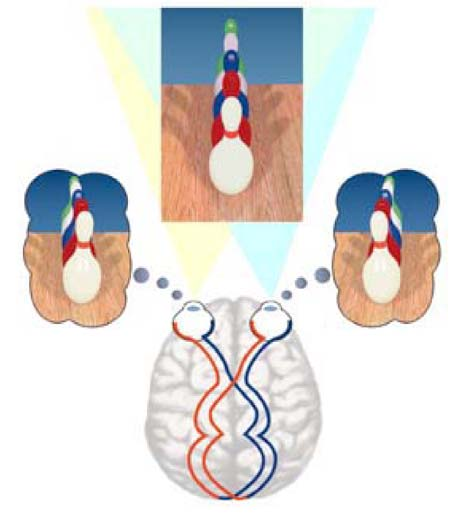
\includegraphics[scale=0.3]{4-Conteudo-Bibliografico/2-Visao-Computacional/Imagens-Visao-Computacional/visao-humana.png}
	\end{center}
	\centering \legend{Fonte: \citeonline{PERONTI2008}}
\end{figure}

\citeonline{PERONTI2008} explica em seu artigo que estereoscopia é a visualização feita por dois mecanismos de captura de imagem em um mesmo foco (\autoref{fig_visao-computacional-camera}).

\begin{figure}[h]
	\caption{\label{fig_visao-computacional-camera}Mecanismos para captação de imagens com focos visuais coincidentes.}
	\begin{center}
		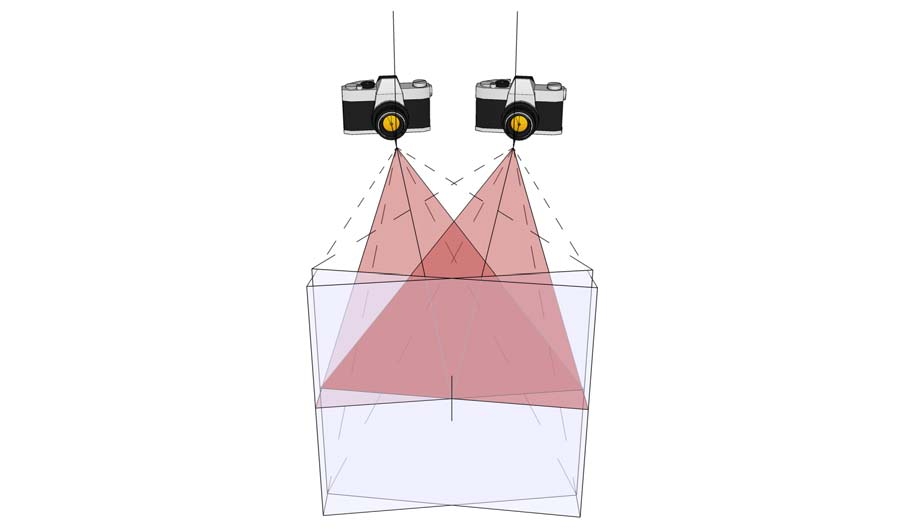
\includegraphics[scale=0.4]{4-Conteudo-Bibliografico/2-Visao-Computacional/Imagens-Visao-Computacional/visao-computacional-camera.png}
	\end{center}
	\centering \legend{Fonte: \citeonline{PERONTI2008}}
\end{figure}

Segundo \citeonline{REHEM2009}, devido ao avanço tecnológico, desenvolveram-se computadores com maior capacidade de processamento gráfico, proporcionando ferramentas com um potencial maior na área de visão computacional. Pode-se dizer que essas ferramentas são bibliotecas onde o seu código fonte é constituído de um agrupamento de funções que potencializam o processamento gráfico de imagens e vídeos. Sendo assim, ao utilizar essas bibliotecas, tem-se a possibilidade de desenvolvimento de técnicas de aperfeiçoamento gráfico para realizar rastreamento de movimentos e de características humanas em tempo real.


\subsection{Captura e identificação de imagem}

A tecnologia vem crescendo cada vez mais em todo mundo, proporcionando a ampliação do uso de dispositivos de alto desempenho. Paralelo a isso, o fluxo de dados aumenta proporcionalmente, exigindo uma velocidade de conexão maior com a Internet. Um exemplo disso são os \textit{smartphones}, que se popularizaram por serem dispositivos multifuncionais, podendo ser utilizados para tarefas profissionais e pessoais. 

Por conseguinte deste avanço científico, é notório a grande evolução na utilização de imagens digitais em várias áreas, como, por exemplo, em transmissões de TV, conteúdos via streaming, imagens capturadas por satélite e até mesmo imagens transmitidas pelas redes sociais. No entanto, como funciona a captura de uma imagem em tempo real? Qual o conceito de imagem?

Uma imagem digital pode ser considerada como sendo uma matriz de pontos elementares, em que cada ponto recebe o nome de \textit{pixel}. Quanto maior a quantidade de \textit{pixels} melhor a resolução da imagem e consequentemente maior o seu tamanho. Cada \textit{pixel} é representado por um valor que indica a intensidade de brilho, denominado nível de cinza, e a quantidade de níveis de cinza depende da quantidade de bits usada na representação de cada \textit{pixel} \cite{SOUZA2007}.

Sendo assim, a matriz de pontos elementares de uma imagem digital pode ser representada conforme na \autoref{fig_imagem-digital-monocromatica}.

\begin{figure}[h]
	\caption{\label{fig_imagem-digital-monocromatica}Representação de uma imagem digital.}
	\begin{center}
		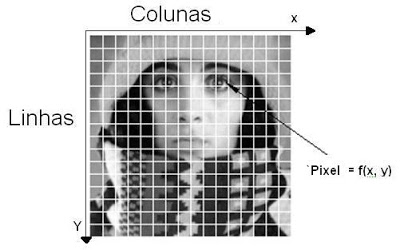
\includegraphics[scale=0.5]{4-Conteudo-Bibliografico/2-Visao-Computacional/Imagens-Visao-Computacional/imagem-digital-monocromatica.JPG}
	\end{center}
	\centering \legend{Disponível em: http://sdbmcc.blogspot.com/2009/06/imagem-digital-teoria.html}
\end{figure}

A captura e identificação em tempo real de uma imagem consiste em analisar um ambiente tridimensional e elaborar digitalmente uma imagem 2-D (Duas dimensões), ocasionando uma imagem estática daquele ambiente tridimensional selecionado. Esse conceito está relacionado a perspectiva, segundo \citeonline{PERONTI2008}. Para que isso seja possível, é necessário utilizar um dispositivo capaz de realizar essa ação, ou seja, uma câmera digital, \textit{smartphones}, dentre outros.

Segundo \citeonline{CHMIELEWSKI2009}, isso se tornou capaz devido a uma tecnologia que surgiu nos anos 70 denominada CCD, \textit{Charge Coupled Device} (Dispositivo acoplado de carga): “O sensor CCD ou dispositivo de carga acoplada é uma matriz de elementos sensíveis à luz, fabricados utilizando tecnologia MOS, \textit{Metal Oxide Semiconductor} (Semicondutor de óxido metálico), onde cada \textit{pixel} pode ser considerado como um capacitor MOS.”

Atualmente, o sensor mais utilizado nos dispositivos de captura de imagem são de sistemas digitais CMOS - \textit{Complementary Metal Oxide Semiconductor} (Semicondutor complementar de óxido metálico), que surgiu nos anos 90 devido a um protótipo do sensor de imagem APS - \textit{Active Pixel Sensor} (Sensor de pixel ativo) criado pela NASA - \textit{National Aeronautics and Space Administration} (Administração Nacional Aeronáutica e Espacial), que possibilitou a fabricação direta de funções como \textit{zoom}, diferentes resoluções de aquisições, acesso aleatório, etc., podendo executar todas as funções do CCD. “Os sensores de imagem APS são formados por elementos sensíveis à luz, capazes de gerar um sinal elétrico ou carga proporcional à intensidade da luz que incide sobre eles.” \cite{CHMIELEWSKI2009}

\subsection{Processamento de imagem}

O grande marco da área de processamento de imagens aconteceu no século XX com o surgimento dos primeiros computadores digitais com grande capacidade de processamento e o início do programa espacial norte-americano, ocorreu um grande impulso na área de processamento de imagem. O uso de técnicas computacionais de aprimoramento de imagens teve início no \textit{Jet Propulsion Laboratory} (Laboratório de Propulsão a Jato), localizado no centro tecnológico da NASA, em 1964, quando "imagens da lua transmitidas por uma sonda Ranger eram processadas por computador para corrigir vários tipos de distorção inerentes à câmera de TV acoplada à sonda". Essa tecnologia foi usada em grandes expedições tripuladas, como a Apollo \cite{FILHO1999}.

Para realizar o processamento de uma imagem, são definidos passos a serem seguidos para a garantia do objetivo final. A captura da imagem consiste no uso de dispositivos físicos sensíveis a espectros de energia eletromagnética que convertem o sinal elétrico para um formato digital. O pré-processamento consiste no realce da imagem para enfatizar características de interesse ou recuperar imagens que sofreram alguma degradação devido à introdução de ruído, perda de contraste ou borramento. A segmentação é a extração ou identificação dos objetos contidos na imagem, separando a imagem em regiões. Por fim, a classificação, é o processo que identifica a imagem observada \cite{GONZALEZ2002}.

As etapas básicas do processamento de imagem estão representadas através da \autoref{fig_etapas-processamento-imagem}.

\begin{figure}[h]
	\caption{\label{fig_etapas-processamento-imagem}Etapas básicas do processamento de imagens.}
	\begin{center}
		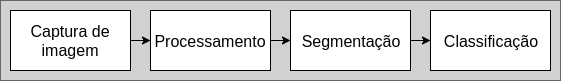
\includegraphics[scale=0.7]{4-Conteudo-Bibliografico/2-Visao-Computacional/Imagens-Visao-Computacional/etapas-processamento-de-imagem.png}
	\end{center}
	\centering \legend{Fonte: Adaptada de \citeonline{GONZALEZ2002}}
\end{figure}

Seres humanos conseguem distinguir vários padrões de cores com certa facilidade, levando em consideração que a análise é feita em um ambiente tridimensional. Na computação, esse discernimento de cores são mais complexos, independentemente da dimensão na qual a imagem será analisada. Isso ocorre porque vários fatores podem contribuir para a má performance computacional no tratamento da imagem, como por exemplo a falta ou excesso de luz, qualidade do sensor, qualidade da imagem, dentre outros.

\begin{citacao}
“Objetos que emitem luz visível são percebidos em função da soma das cores espectrais emitidas. Tal processo de formação é denominado aditivo. O processo aditivo pode ser interpretado como uma combinação variável em proporção de componentes monocromáticas nas faixas espectrais associadas às sensações de cor verde, vermelho e azul, as quais são responsáveis pela formação de todas as demais sensações de cores registradas pelo olho humano. Assim, as cores verde, vermelho e azul são ditas cores primárias. Este processo de geração suscitou a concepção de um modelo cromático denominado RGB (Red, Green, e Blue), para o qual a Comissão Internacional de Iluminação (CIE) estabeleceu as faixas de comprimento de onda das cores primárias.” \cite{QUEIROZ2006}
\end{citacao}

Cada \textit{pixel} é representado por um valor numérico que corresponde a sua cor em questão. Sendo assim, para que seja possível representar uma imagem em alguma escala de cor monocromática (preto e branco, ou escalas de cinza), basta associar o \textit{pixel} a um valor numérico relacionado a sua escala de tom.

A \autoref{fig_rep-pixel-monocromatico} exemplifica a associação dos \textit{pixels} de forma a obter uma imagem monocromática. Segundo \citeonline{NELMA2000}, para obter uma imagem em tons de cinzento, basta associar cada \textit{pixel} um valor inteiro não negativo de um byte, onde o valor 0 corresponde a cor preta e o valor máximo, 255, corresponde a cor branca. Os valores intermediários correspondem aos variados tons de cinza.

\begin{figure}[h]
	\caption{\label{fig_rep-pixel-monocromatico}Imagem médica digital em escalas de cinza (\textit{pixels} monocromáticos).}
	\begin{center}
		\resizebox{.8\linewidth}{!}{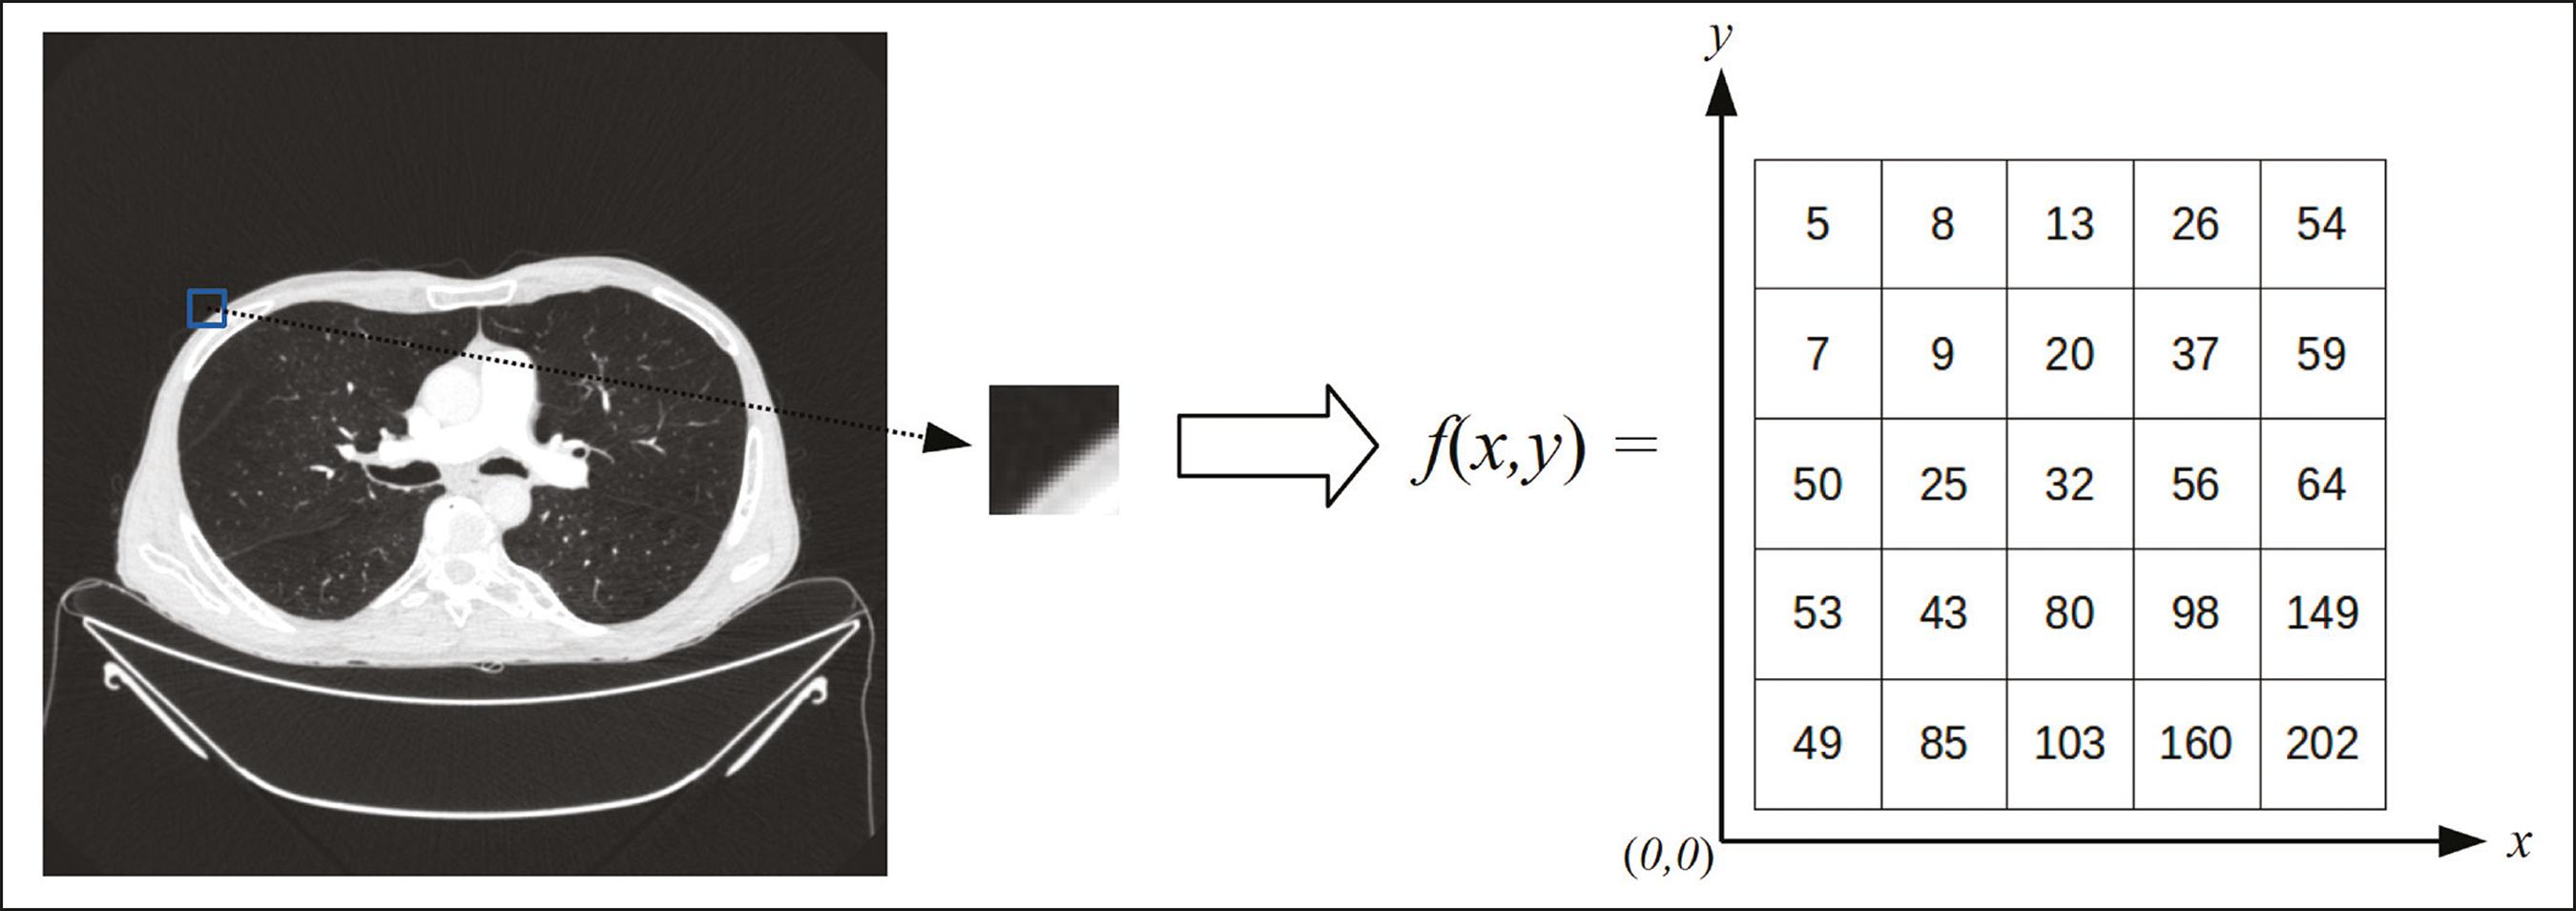
\includegraphics{4-Conteudo-Bibliografico/2-Visao-Computacional/Imagens-Visao-Computacional/repr-pixel-monocromatico.jpg}}
	\end{center}
	\centering \legend{Fonte: \citeonline{SANTOS2019}}
\end{figure}

Já as imagens coloridas exigem um poder maior de processamento para serem reconhecidas. Isso ocorre porque as imagens em RGB - \textit{Red, Green, and Blue} (Vermelho, Verde e Azul)  precisam de mais de uma banda\footnote{Cada matriz ou conjunto de cor diferente é denominado banda de cor. Subconjuntos de três bandas espectrais azul, vermelha e verde compõem uma imagem RGB. Em imagens monocromáticas (Preto e branco), o objeto é representado em apenas uma banda espectral \cite{CROSTA1999}. \label{Banda-de-Cor}} para serem processadas, ou seja, são analisadas três matrizes de cores para formar a paleta de cor específica do tom capturado (\autoref{fig_rgb-representacao}). Depois da análise, são formadas as cores distintas que compõe a imagem.

\begin{figure}[h]
	\caption{\label{fig_rgb-representacao}Matriz de \textit{pixels} RGB.}
	\begin{center}
		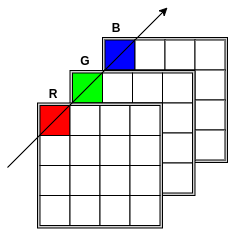
\includegraphics[scale=0.6]{4-Conteudo-Bibliografico/2-Visao-Computacional/Imagens-Visao-Computacional/matriz-de-pexels-rgb.png}
	\end{center}
	\centering \legend{Fonte: Elaborada pelos autores do projeto.}
\end{figure}

De forma mais detalhada, \citeonline{LOPES2013} exemplificam que imagens coloridas também são imagens multibanda, ou multiespectral. As cores visíveis através de olhos humanos podem ser representadas pela combinação de bandas das cores primárias vermelha, verde e azul (\textit{Red, green} e \textit{blue}, respectivamente). A imagem colorida também pode ser armazenada por meio de imagens cromáticas e mapas de cores. Nesse caso, o valor de cinza de cada \textit{pixel} na imagem se torna um índice para uma entrada de mapa de cores, enquanto a entrada em si do mapa de cores contem os valores dos componentes referentes as tonalidades \textit{RGB} (\autoref{fig_rep-pixel-rgb}).

\begin{figure}[h]
	\caption{\label{fig_rep-pixel-rgb}Imagem digital em tons coloridos (\textit{pixels} RGB).}
	\begin{center}
		\resizebox{.6\linewidth}{!}{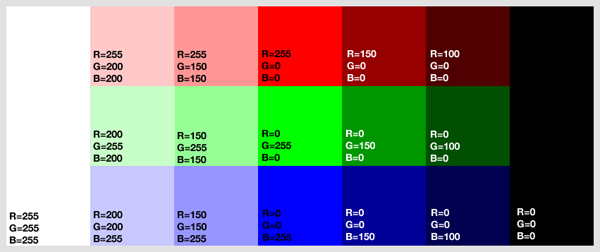
\includegraphics{4-Conteudo-Bibliografico/2-Visao-Computacional/Imagens-Visao-Computacional/repr-pixel-rgb.jpg}}
	\end{center}
	\centering \legend{Disponível em: https://apenasimagens.com/pt/pixel-imagem-digital/}
\end{figure}

No entanto, a imagem capturada por algum dispositivo eletrônico pode chegar de forma irregular ate a parte de processamento. Essas falhas podem ser caracterizadas de várias formas, como por exemplo a presença de \textit{pixels} ruidosos, brilho e/ou contrastes desregulados, caracteres com dígitos incompletos ou apagados como em digitalizações de documentos.

A parte de processamento fica responsável por elaborar uma melhoria da imagem em questão, ajustando todos os parâmetros para que seja possível analisar precisamente todas as informações que estão disponíveis no arquivo de imagem. Sendo assim, por analogia as imagens processadas, trata-se de uma etapa que analisa de forma profunda todos os dados contidos na imagem, ou seja, a fase de processamento abrange os níveis mais baixos de análise de imagens, pois trabalham diretamente com valores de intensidade dos \textit{pixels}, visto que neste período não existe nenhuma informação relacionada a imagem para que seja possível facilitar o trabalho.

\subsubsection{\textit{Segmentação de imagens}}

De forma a dar continuidade ao ciclo de processamento de imagem e verificação desta, usa-se métodos de \textit{pixels} e tonalidades seguindo os padrões propostos. A análise deve prosseguir de forma minuciosa para então, processar seus detalhes.

A segmentação veio para aprimorar a parte de processamento, auxiliando na detecção de maiores detalhes e reduzindo tempo de processamento. Isso ocorre porque a segmentação é a área que tem por responsabilidade dividir a imagem em várias partes significativas, separando as de interesse dentro desta \cite{FILHO1999}.

No entanto, a segmentação exige um processamento muito grande para analisar a imagem sugerida. Sendo assim, o nível no qual será feito essa subdivisão de imagem depende muito da ocasião e do problema que está sendo proposto para resolver. De acordo com \citeonline{GONZALEZ2002}, para não ocorrer perca desnecessária de processamento e, consequentemente, perda de tempo, a segmentação deve parar assim que os objetos de interesse da aplicação forem isolados.

Portanto, dentro da segmentação existem métodos que podem ser seguidos a fim de analisar detalhadamente cada figura. Segundo \citeonline{MORGAN2008}, as classificações dos métodos utilizados na segmentação são definidos como interativos ou automáticos. Basicamente, a diferença entre os dois são bem simples: um é executado através de intervenções humanas e o outro não.

Além disso, no processo de segmentação interativa, o usuário utiliza ferramentas e técnicas que se adéquam da melhor forma a sua imagem e necessidade, solucionando-a da melhor forma possível. Esse método normalmente é mais utilizado para solucionar problemas específicos, onde as condições da imagem podem interferir drasticamente na análise final da mesma como, por exemplo, \textit{softwares} que analisam imagens de doenças graves adquiridas através de ressonâncias, onde a aplicação pode confundir um ruído ou uma área com má iluminação em um ponto de análise clínica.

Já o processo de segmentação automática onde, na maioria das vezes, utilizam robôs para realizar as tomadas de decisões através dos resultados obtidos na análise da imagem, inexiste interferência humana no processo. Esse método está sendo aplicado, por exemplo, em carros autônomos, onde o mesmo identifica a presença de obstáculos em sua frente e com base no obstáculo e na proporção do mesmo, uma ação e tomada.

Para complementar, \citeonline{MORGAN2008} enfatiza que existem métodos que são classificados de acordo com a representação dos objetos a serem segmentados, que são os métodos de borda ou orientados a regiões.

O processo de segmentação baseado no método de bordas utiliza basicamente pontos de uma imagem onde ocorre alguma intensidade de luz, ou seja, onde os \textit{pixels} estão mais visíveis, realçando a borda do objeto e consequentemente diferenciando do fundo da imagem. Pode-se também localizar uma borda através de uma mudança brusca nos tons de cinza, gerados por regiões distintas. Com base na borda que foi extraída da imagem, tem-se então uma imagem topográfica do objeto que será analisado.

A \autoref{fig_metodo-de-borda} mostra como funciona uma análise baseada no método de bordas.

\begin{figure}[h]
	\caption{\label{fig_metodo-de-borda}Resultado de uma análise feita utilizando o método de bordas.}
	\begin{center}
		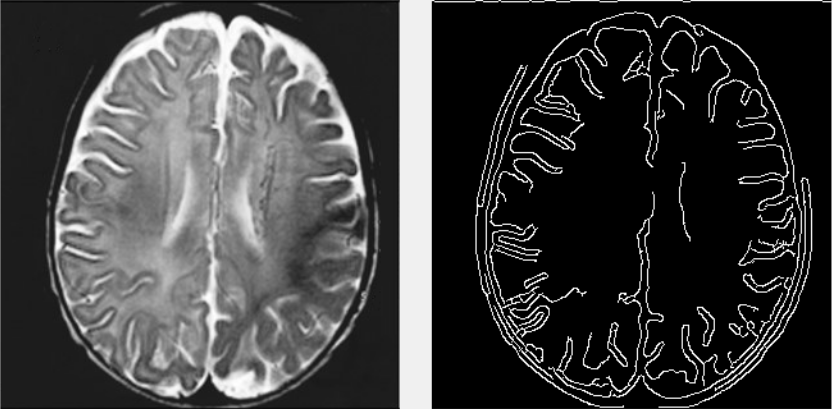
\includegraphics[scale=0.3]{4-Conteudo-Bibliografico/2-Visao-Computacional/Imagens-Visao-Computacional/metodo-de-borda.png}
	\end{center}
	\centering \legend{Fonte: \citeonline{FREITAS2016}}
\end{figure}

Conforme \citeonline{MORGAN2008} enfatiza em seu artigo, o método orientado a regiões é dividido em três abordagens relevantes: classificação por \textit{pixel}, agregação de \textit{pixel} e \textit{split-and-merge} (Divisão e conquista).

A descrever cada uma das abordagens de forma didática, a classificação por \textit{pixel} nada mais é que a identificação de características presentes na imagem como, por exemplo, cor, texturas, a fim de classificar os \textit{pixels} de acordo com as várias possibilidades de classes ou objetos da imagem.

Na abordagem de agregação por \textit{pixel} o objetivo é encontrar um \textit{pixel} dentro da imagem e, a partir desse \textit{pixel}, ocorre o crescimento de regiões conexas. O desenvolvimento das regiões acontece ate alcançar o critério de parada do crescimento, onde estará representado um objeto dentro da imagem.

Já a segmentação utilizando a bordagem \textit{split-and-merge} é mais complexa. Segundo \citeonline{VENTURA2009}, ao aplicar essa abordagem de segmentação, o objetivo final consiste em conseguir subdividir a imagem em vários quadrantes que satisfaça uma prioridade. Apos a concretização desta tarefa, realiza-se a verificação de cada quadrante, observando se este atende ou não a prioridade definida. Caso o quadrante não satisfaça a prioridade, a subdivisão acontece novamente em busca de outros quadrantes.

Por fim, o processo de fusão é realizado, acontecendo então o agrupamento das partes similares, ou seja, que atende as prioridades definidas. Esse processo só finaliza quando não existe nenhuma possibilidade de realizar divisões ou agrupamentos.

\subsubsection{\textit{Histograma}}

O histograma é um método que auxilia na identificação de objetos e/ou características específicas da imagem, obtendo uma maior precisão nos resultados obtidos.

Segundo \citeonline{FILHO1999}, histogramas são conjuntos de vários números no qual são indicados os percentuais de \textit{pixels} de uma imagem que possui determinados níveis de cinza. Estes valores, normalmente representados por gráficos, apresentam, para cada nível de cinza, o seu percentual de \textit{pixels} correspondente na imagem. Com base nessa análise feita pelo histograma, pode-se obter os níveis de contraste, brilho, e até mesmo informações de predominância clara ou escura.

\citeonline{FILHO1999} explicam que, através de equações matemáticas, é possível obter um resultado satisfatório ao analisar cada elemento deste conjunto. Este trabalho não tem por finalidade apresentar e/ou explicar cálculos matemáticos que cada função executa.

De forma a complementar o assunto, \citeonline{MAIZA2013} expressa em sua tese que, ao obter o histograma da imagem, pode-se alcançar medidas estatísticas dos níveis de cinza da imagem, como por exemplo o seu valor mínimo e máximo, valor médio, variância e desvio padrão. Portanto, o histograma seria como um método de probabilidade, onde o número de \textit{pixels} de um determinado nível de cinza pode ser utilizado para calcular um outro \textit{pixel} com o mesmo valor de cinza na imagem (\autoref{fig_histograma}).

\begin{figure}[h]
	\caption{\label{fig_histograma}Imagem (a) e seu respectivo histograma (b).}
	\begin{center}
	\resizebox{.8\linewidth}{!}{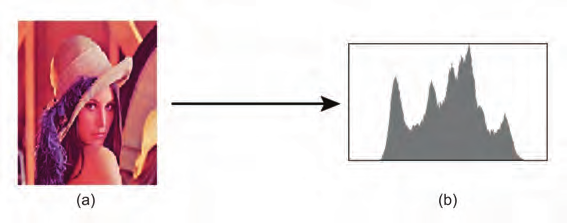
\includegraphics{4-Conteudo-Bibliografico/2-Visao-Computacional/Imagens-Visao-Computacional/histograma.png}}
	\end{center}
	\centering \legend{Fonte: \citeonline{MAIZA2013}}
\end{figure}

\subsubsection{\textit{Classificação de imagens}}
\label{classificacao-de-imagem}
% \textbf coloca o subsection em negrito

A classificação de imagem é a última etapa do processamento de imagem (\autoref{fig_etapas-processamento-imagem}). Em síntese, esta etapa é responsável por realizar a classificação das imagens levando em consideração as suas características.

Entretanto, segundo \citeonline{LIBERMAN97}, nessa etapa do processamento, o grau de abstração de cada característica da imagem pode ser classificado em três níveis distintos: baixo, médio e alto.

No processo de baixo nível são utilizados os \textit{pixels} originais da imagem como parâmetros de comparação, para que no final do processo sejam gerados propriedades da imagem, em forma de valores numéricos, associadas a cada \textit{pixel} que foi analisado. Sequencialmente, o nível médio coleta essas propriedades numéricas geradas pelo processo de baixo nível e produz uma lista de características da imagem. Por fim, o processo de alto nível reúne estas características ocasionadas pelo processo anterior buscando interpretá-las, formando assim o conteúdo da imagem.

Segundo \citeonline{LIBERMAN97}, o processo de classificação ou interpretação de uma imagem é a parte mais inteligente da visão computacional. O autor do artigo cita que essa é uma das etapas de maior nível, no qual permite-se obter a “compreensão e a descrição final do fenômeno inicial”.

Para complementar, \citeonline{LIBERMAN97} explica que o processo de classificação de imagem possui duas técnicas para realizar suas tarefas, sendo divididas em supervisionada ou não-supervisionada. A classificação não-supervisionada consiste em um agrupamento automático de sequências similares de uma imagem analisada. Conforme já prescrito neste trabalho no contexto de segmentação interativa e agora completado por \citeonline{LIBERMAN97}, nessa etapa a imagem será segmentada em um número indeterminado de classes, no qual o usuário também será responsável por gerenciar essas classes a fim de alcançar seus objetivos.

De acordo com \citeonline{MAXIMO2005}, no processo de classificação supervisionada, o analista ou usuário filtra as classes de informações seguindo os seus padrões de interesse e separa, na imagem, as regiões que satisfazem essas classes. Após a delimitação das classes, a técnica analisará as mesmas com o objetivo de delimitar \textit{pixels} que serão utilizados como parâmetros para a busca de demais \textit{pixels}.

Simplificadamente, a técnica de classificação supervisionada utiliza amostras de características coletadas durante o processo para identificar cada \textit{pixel} definido como \textit{pixel} desconhecido, ou seja, tons de \textit{pixels} que não fazem parte das características já coletadas anteriormente seguindo os filtros definidos pelo usuário.

\input{4-Conteudo-Bibliografico/2-Visao-Computacional/haar-cascade.tex}

\input{4-Conteudo-Bibliografico/2-Visao-Computacional/machine-learning.tex}

\subsubsection{\textit{Similaridade}}

De forma concisa, similaridade consiste em realizar uma buscar dentro de uma imagem específica com o objetivo de reconhecer/encontrar objetos semelhantes a um modelo de busca. Nessas funções de busca por similaridade são utilizados cálculos de vetores de características para realizar as comparações de igualdade \cite{MAIZA2013}.

Os seres humanos possuem uma grande facilidade de reconhecer informações apresentadas de maneira visual, onde consequentemente são capazes, com grande facilidade, de interpretar imagens diversificadas sem grande esforço. Exemplificando esta situação, os seres humanos consegue distinguir de forma fácil a diferença entre um círculo grande e um círculo pequeno, um quadrado grande de um quadrado pequeno, a diferença entre um triângulo e um quadrado de tamanhos idênticos, dentre outros. Conforme \citeonline{SILVA2009} relata em seu artigo, com a tecnologia disponível atualmente para realizar a construção de aplicações capazes de identificar informações dentro de uma imagem ainda é muito ineficiente, quando comparada com a capacidade humana.

Segundo \citeonline{MAIA2013}, algoritmos de similaridade trabalham com métricas que informam o quanto uma imagem é parecida com a outra. Ou seja, pode-se aplicar essas métricas utilizando padrões de buscas a fim de uma análise mais específica. De forma estatística, \citeonline{MAIA2013} completam que possui dois tipos básicos de medidas de similaridade: correlação e coseno. Seguindo o contexto do artigo, a similaridade por correlação entre dois vetores retorna um valor booleano, ou seja, 0 e 1, onde o valor de retorno igual a 1 significa que há uma similaridade forte naquele ponto, ou seja, os valores dos vetores são parecidos e, se o retorno for 0, não existe correlação. No entanto, o autor enfatiza a presença de um retorno igual a -1, no qual a similaridade daquele ponto é inversa ao padrão de busca. Ja a similaridade por coseno é similar a correlação, no qual o retorno também e 0 e 1, porém nesse método é analisado o tamanho do vetor e a formação de um ângulo entre os mesmos. Quanto mais próximo de 1 for o valor, mais similares são os vetores.

\citeonline{MAIZA2013}, \citeonline{MAIA2013} utilizam em seus artigos a função euclidiana para realizar cálculos de distâncias nas estruturas. Essa função utiliza métricas de similaridade para calcular a distância entre dois vetores de características, percorrendo o vetor apenas uma vez. A distância euclidiana entre dois pontos (Xi e Xj) é definida através de uma equação matemática, na qual não faz parte do escopo deste projeto.

\subsection{Reconhecimento facial}

Dentre as diversas tarefas que os computadores podem executar, o reconhecimento facial tem tido uma crescente, se tornando alvo de vários estudos. Algoritmos de reconhecimento facial estão presente em diversos dispositivos, como por exemplo \textit{smartphones} e câmeras digitais, e ate mesmo carros autônomos, que escaneiam seus obstáculos para realizar uma tomada de decisão. Grandes aperfeiçoamentos dentro desta área estão sendo implementados de forma gradativa com a finalidade de realizar análises com grandes precisões e mais próximas a visão humana.

Segundo \citeonline{SZELISKI2010}, a área de reconhecimento facial foi a que teve mais sucesso nos dias atuais. No entanto, a aplicação desse algoritmo para realizar a busca de uma pessoa dentro de milhares de pessoas em tempo real, ainda é um desafio para a tecnologia, embora pra humanos essa tarefa também é bem difícil. Mas quando esse grupo de pessoas é reduzido a, por exemplo, um grupo familiar ou grupo de amigos, a ferramenta tem um desempenho excepcional. O objeto na qual esta sentá sendo utilizado para ler o ambiente físico, ou seja, o dispositivo de captura de imagem, influencia diretamente com o desempenho da ferramenta.

Sendo assim, o resultado do reconhecimento facial pode ser intensificado quando a imagem é capturada de forma frontal as pessoas, no qual seja possível localizar por completo os rostos das pessoas em questão. Porem, vários fatores podem interferir na análise da imagem, por exemplo: iluminação, qualidade dos sensores, dentre outros fatores de interferência. Para tentar solucionar esses problemas, uma das primeiras abordagens a ser seguida pela ferramente e tentar analisar os locais de características específicas da imagem como, por exemplo, nariz, boca, olhos, e aplicar medidas de distância entre os pontos de características encontrados \cite{SZELISKI2010}.

Existem várias ferramentas que proporcionam ao usuário utilizar a tecnologia de visão computacional para realizar o reconhecimento facial. Dentre estas ferramentas, a biblioteca OpenCV disponibiliza funções capazes de reconhecer objetos e pessoas. 

\section{\textbf{{Engenharia de \textit{software}}}}
\label{engenharia-software}

Quando se pensa em desenvolvimento, manutenção, especificação e criação de um \textit{software}, pensa-se também em tecnologias e práticas de gerência de projetos para que a execução da aplicação aconteça de forma organizada, produtiva e com a máxima qualidade possível. Tudo isso esta contido em engenharia de \textit{software}.

Segundo \citeonline{PRESSMAN2016} em seu livro, um \textit{software} bem sucedido é aquele que atende a todos os requisitos do usuário, fica implementado durante um bom tempo, é de fácil manutenção e operabilidade. Por outro lado, um \textit{software} mal sucedido pode acarretar diversos fatos desagradáveis, levando os usuários a insatisfação e ao erro. 

Apesar de gerentes, líderes de projetos e profissionais envolvidos com a área técnica entenderem a necessidade de uma metodologia mais disciplinar no desenvolvimento de \textit{softwares}, existe ainda discursos de como e qual é a melhor metodologia a ser aplicada no projeto. Essa indecisão ocorre devido a grande demanda de produção que acontece atualmente, principalmente no setor de desenvolvimento de aplicações. Outro impacto negativo, é o fato de que profissionais e empresas começam a desenvolver \textit{softwares} de forma descontrolada mesmo com uma metodologia organizacional aplicada, justamente por não estarem preparados para uma abordagem disciplinar \cite{PRESSMAN2016}. 

Com base nisso, a engenharia de \textit{software} evoluiu rigorosamente, passando de uma simples técnica implementada por um publico relativamente pequeno para uma comunidade que objetiva o planejamento e a organização ates de iniciar qualquer tipo de desenvolvimento.

Sendo assim, em 2001, o engenheiro de \textit{software} Kent Beck juntamente com os principais
desenvolvedores de métodos ágeis, assinaram o “Manifesto para o Desenvolvimento Ágil de Software” \cite{SOMMERVILLE2011}, que tem por iniciativa a seguinte ideia:

\begin{citacao}
"Estamos descobrindo melhores maneiras de desenvolver \textit{software}, o fazendo e ajudando outros a fazê-lo. Através desse trabalho, valorizamos mais:

Indivíduos e interações do que processos e ferramentas;\\
\textit{Software} em funcionamento do que documentação abrangente;\\
Colaboração dos clientes acima de negociação contratual;\\
Respostas a mudanças acima de seguir um plano;\\
Ou seja, embora itens à direita sejam importantes, valorizamos mais os que estão à esquerda.\cite{SOMMERVILLE2011}"
\end{citacao}

\subsection{Engenharia de Requisitos}

Quando se pensa em projetar e construir um \textit{software}, os desafios e as imaginações tomam proporções escalonáveis para obter a melhor forma de iniciar e prosseguir com o desenvolvimento do projeto. O grande problema nesse processo é definir quais são os requisitos necessários para que o sistema atenda as necessidades do usuário.

Segundo \citeonline{PRESSMAN2005}, a engenharia de requisitos é basicamente uma etapa da engenharia de software, que deve ser iniciada durante as atividades de comunicação e continua no decorrer do desenvolvimento do \textit{software}. "Ela deve ser adaptada às necessidades do processo, do projeto, do produto e das pessoas que estão realizando o trabalho.”

A engenharia de requisitos tem por objetivo fornecer regras apropriadas para entender as necessidades do cliente afim de avaliar a viabilidade, negociar soluções razoáveis, validar as especificações e gerenciar as necessidades dos usuários na medida em que o sistema seja desenvolvido \cite{PRESSMAN2016}.

\subsection{{Desenvolvimento ágil de \textit{software}}}

Quando se pensa em desenvolvimento de \textit{software}, deve-se reconhecer que o processo é bem instável e com baixa previsibilidade, se tornando algo complicado de estabelecer métricas a serem seguidas. Vários pontos de interferência pode intervir para que um \textit{software} não possa ser desenvolvido da maneira correta, como por exemplo uma equipe de trabalho desestruturada, nos quais os integrantes não possuem uma boa convivência entre si, ou uma metodologia de desenvolvimento sem uma linha cronológica a ser seguida. Reconhecer que este é um grande desafio é algo sensato de se fazer. No entanto existem mecanismos de correção para melhorar o processo de desenvolvimento.

A metodologia ágil surgiu para organizar esses processos de desenvolvimento de \textit{software}, elaborando uma padronização nos projetos para que seja possível otimizar os fluxos de trabalho e melhoras a produtividade do projeto. Segundo \citeonline{SOARES2004}, a principal característica da metodologia ágil e que ela pode ser adaptada, ao invés de ser preditiva. Ou seja, se ocorrer algum problema no decorrer do desenvolvimento, a própria metodologia é flexível o bastante para contornar a situação e prosseguir com o desenvolvimento do projeto. Portanto, uma empresa pode facilmente criar a sua própria metodologia de trabalho, seguindo a sua experiência empresarial, analisando os seus acertos e erros para elaborar um procedimento que se adéqua as suas necessidades. 

\citeonline{SOARES2004} continua exemplificando que a metodologia ágil trabalha com constantes \textit{feedbacks} e reuniões, nas quais permitem aos membros da equipe expor as facilidades e dificuldades de suas tarefas, bem como o seu status de desenvolvimento. A partir destes \textit{feedbacks}, o gestor pode traçar a melhor maneira de organizar a equipe para que os membros com maior experiência deem apoio nas dificuldades apresentadas pelos outros integrantes da equipe. Outro grande motivo expressado no contexto é o fato ocorrer entregas constantes de partes operacionais do software. Desta maneira, o usuário final do software pode ter uma prévia de como o sistema está sendo desenvolvido, bem como suas funcionalidades e \textit{design}, podendo solicitar alguma possível alteração ou identificar algum problema antes da implantação oficial dos modulos.

\input{4-Conteudo-Bibliografico/3-Engenharia-Software/kanban.tex}

\input{4-Conteudo-Bibliografico/3-Engenharia-Software/trello.tex}

\section{\textbf{Ferramentas de desenvolvimento do projeto}}
\label{ferramentas-de-desenvolvimento-do-projeto}

Em relação as ferramentas de desenvolvimento, é notório que existe um trajeto amplo a ser percorrido pelos programadores. Isso ocorre porque existem várias linguagens de programação e \textit{frameworks} que auxiliam no desenvolvimento de sistemas. A escolha da melhor linguagem de programação e o melhor \textit{framework} para desenvolvimento depende muito do problema a ser resolvido e também das habilidades do programador. Há também um grande impasse na escolha da melhor linguagem e/ou do melhor \textit{framework}, que está relacionado a: interesses e aplicações comerciais; comunidade, para esclarecer possíveis dúvidas e curva de aprendizado.

\subsection{{Linguagem de programação}}

Linguagem de programação são codificações escritas sequencialmente, seguindo uma estrutura assíncrona para a resolução de algum problema ou tarefa, que tem por finalidade ser compreendida por um computador. Essas codificações descrevem ao computador a sequência lógica de execução das funções e os comandos nos quais ele deve realizar para que a tarefa e/ou problema seja executado da melhor forma possível. Basicamente são divididas em linguagem de baixo nível e de alto nível, que significam, respectivamente, linguagens próximas ao entendimento de máquina ou \textit{hardware} (Binário ou hexadecimal) e linguagens próximas as linguagens naturais, ou seja, de fácil entendimento humano (\textit{While, if, write, read,} etc), nos quais são necessários compiladores para realizar a tradução, tornando possível a compreensão da máquina \cite{KELLEHER2005}.

Na busca por uma linguagem que poderia satisfazer e tornar possível a construção de uma solução para o impasse explícito no trabalho, fora identificado uma forte tendência na utilização do \textit{Python}.

\begin{comment}
De acordo com \citeonline{PILGRIM2009}, a projeção da linguagem enfatiza o trabalho do programador sobre o computacional, possibilitando assim a construção de bibliotecas e frameworks com uma facilidade acima do normal.

\textit{Python} foi criado por Guido van Rossum em 1991, com a ajuda de seus colegas Jack Jansen e Sjoerd Mullender. O objetivo deles era criar uma linguagem de fácil entendimento, orientada a objetos, menos complexa possível \cite{SONGINI2005}.

Segundo \citeonline{OLIVEIRA2007}, a linguagem sofreu vários ajustes no decorrer dos anos, tornando-se muito popular dentre os desenvolvedores e, consequentemente, dando início a inúmeras aplicações. Portanto, \textit{Python} é uma linguagem orientada a objetos, fortemente tipada, com propositos gerais de alto nível e de código aberto, objetivando uma construção ágil no desenvolvimento de aplicações. Sua sintaxe é bem simples e de fácil entendimento, reduzindo o custo de manutenção em \textit{softwares} criados a partir desta. Suas bibliotecas garantem ao programador um vasto acervo de funções que tem por finalidade facilitar o seu trabalho, reduzir tempo de codificação e evitar arquivos com extensas linhas de código. Devido à comunidade de código aberto, onde desenvolvedores tem acesso ao seu código fonte, a popularização da linguagem vem crescendo de forma significativa, visto que esta ainda não é muito conhecida \cite{SONGINI2005}.
\end{comment}

\subsubsection{\textit{Python}}

De acordo com \citeonline{PILGRIM2009}, a projeção da linguagem enfatiza o trabalho do programador sobre o computacional, possibilitando assim a construção de bibliotecas e frameworks com uma facilidade acima do normal.

\textit{Python} foi criado por Guido van Rossum em 1991, com a ajuda de seus colegas Jack Jansen e Sjoerd Mullender. O objetivo deles era criar uma linguagem de fácil entendimento, orientada a objetos, menos complexa possível \cite{SONGINI2005}.

Segundo \citeonline{OLIVEIRA2007}, a linguagem sofreu vários ajustes no decorrer dos anos, tornando-se muito popular dentre os desenvolvedores e, consequentemente, dando início a enumeras aplicações. Portanto, \textit{Python} é uma linguagem orientada a objetos, fortemente tipada, com propósitos gerais de alto nível e de código aberto, objetivando uma construção ágil no desenvolvimento de aplicações. Sua sintaxe é bem simples e de fácil entendimento, reduzindo o custo de manutenção em \textit{softwares} criados a partir desta. Suas bibliotecas garantem ao programador um vasto acervo de funções que tem por finalidade facilitar o seu trabalho, reduzir tempo de codificação e evitar arquivos com extensas linhas de código. Devido à comunidade de código aberto, onde desenvolvedores tem acesso ao seu código fonte, a popularização da linguagem vem crescendo de forma significativa, visto que esta ainda não é muito conhecida \cite{SONGINI2005}.

\subsubsection{{Biblioteca \textit{OpenCV}}}

Devido aos avanços em estudos científicos tecnológicos na área de visão computacional, o surgimento de bibliotecas que utilizam desta tecnologia evoluiu consideravelmente, proporcionando aos usuários maior versatilidade na escolha da melhor ferramenta para uma possível solução de seus problemas. Dentre as principais ferramentas que implementam algoritmos de visão computacional, pode-se citar as mais utilizadas: \textit{Matlab}, \textit{OpenCV} e \textit{scikit-image}. Este trabalho tem o objetivo de abordar apenas a biblioteca \textit{OpenCV}, no qual será utilizada para o desenvolvimento de uma possível resolução ao problema supracitado. A biblioteca \textit{Open Source} (Código aberto) está disponível no seu site oficial \citeonline{OpenCV}.

Desenvolvida pela Intel no ano 2000, escrita nativamente em C++, a biblioteca OpenCV permite a manipulação de dados de imagens, manipulações vetoriais, rotinas de álgebra linear, desenvolvimento de algoritmos de processamento de imagem, calibração de câmeras, dentre outros. Sua flexibilidade com várias linguagens de programação, como por exemplo o \textit{Python}, permite uma melhor integração com vários programas, evitando possíveis conflitos de incompatibilidade e proporcionando uma melhor flexibilidade no desenvolvimento de \textit{softwares} \cite{BARBOZA2009}.

A bilioteca possui certificação BSD - \textit{Berkeley Software Distribution}, representando que o software possui uma licença gratuita. A biblioteca contem mais de 2.500 algoritmos otimizados com diversas propriedades para resolverem problemas extensos. Há também vários setores de aplicação da biblioteca, visto que esta abrange diversas áreas como, por exemplo, reconhecimento de face e objetos, extração de modelos de objetos tridimensionais, união de imagens em uma única imagem, pesquisar por imagens semelhantes dentro de um banco de dados, acompanhar movimentos dos olhos, reconhecimento de cenários, dentre outros. No site oficial da ferramenta encontra-se dados nos quais informam que esta possui uma comunidade com mais de 47 mil usuários e um número estimado de download que ultrapassa a casa dos 18 milhões \cite{CUNHA2013}.

Segundo \citeonline{CUNHA2013}, um dos objetivos da biblioteca \textit{OpenCV} é fornecer uma infraestrutura robusta na área de visão computacional na qual seja de fácil manipulação, ajudando os desenvolvedores no processo de ampliação de aplicações sofisticadas de visão.

%\subsubsection{\textit{Framework}}

Atualmente, os projetos de desenvolvimento de \textit{software} aumentou consideravelmente. Devido a isso, programadores se deparam com um excesso de funções similares dentro dos vários projetos desenvolvidos no decorrer do tempo. Sendo assim, surgiu a necessidade de reutilizar códigos para poupar tempo. 

De acordo com \citeonline{JOHNSON97}, \textit{framework} são estruturas desenvolvidas com o objetivo de reutilizar tudo ou parte de um sistema representado por um conjunto de classes abstratas e concretas, ou seja,  uma estrutura parcialmente completa projetada para ser instanciada. Existe também \textit{frameworks}  que disponibilizam \textit{templates} como base para iniciar o desenvolvimento.

Os \textit{frameworks} disponibilizam para os desenvolvedores um vasto conjunto de bibliotecas, permitindo assim a realização de operações de grande porte. Sendo assim, os programadores focam mais em resolver problemas do que reescrever códigos, aumentando consideravelmente a produtividade da equipe. 

\subsection{{Ambientes virtuais}}

A virtualização vem sendo muito utilizada na área de desenvolvimento de \textit{software} devido à sua flexibilidade e fácil manipulação para realizar a criação de ambientes virtuais. Isso ocorre porque, com a virtualização, o usuário pode criar vários ambientes virtuais e, dentro deles, realizar a instalação das dependências necessárias para a execução do projeto. Portanto, o desenvolvedor pode ativar e desativar o ambiente virtual assim que necessário, sendo que as dependências do projeto estarão instaladas somente nesse ambiente, e não globalmente na máquina. Ou seja, as dependências do projeto serão desativadas assim que a virtualização for encerrada. A utilização de virtualização permite ainda que recursos computacionais possam ser alocados para múltiplas aplicações simultaneamente, sendo que cada uma dessas aplicações possui seu ambiente isolado das demais.

A situação citada acima é bastante válida se analisarmos o crescimento de ferramentas de programação disponíveis atualmente. Instalar vários \textit{frameworks}, pacotes de dependências de linguagens, bibliotecas e afins globalmente na máquina pode acarretar a lentidão, conflitos entre versões de linguagens de programação e \textit{frameworks} dos projetos, dentre outros. Quando isso acontece, por exemplo, em um projeto feito por uma equipe, a atualização de todas as dependências deve ser feita em todas as máquinas que estão envolvidas no projeto, para que a versão seja padrão em toda a equipe.

\subsection{{Sistema de controle de versões}}

Durante o processo de desenvolvimento de \textit{software}, a etapa de codificação gera várias linhas de códigos. Além disso, modificações e melhorias no \textit{software} ocorrem constantemente no decorrer do tempo, seja a pedido do usuário ou alguma possível atualização.  As equipes de desenvolvimento são compostas por vários tipos de desenvolvedores, cada um com sua personalidade e experiência. Sendo assim, os desenvolvimentos de \textit{softwares} são feitos por etapas, onde cada desenvolvedor é responsável por entregar o que foi designado a ele. 

Devido a isso, para organizar essas etapas de desenvolvimento, utiliza-se ferramentas que gerencia e controla diferentes versões de \textit{software}.  Segundo \citeonline{OReilly},  uma ferramenta que realiza o gerenciamento e o controle de versões de \textit{software} ou outro conteúdo “é referida genericamente como um VCS - \textit{Version Control System} (Sistema de controle de versão ), um SCM - \textit{Source Code Manager} (Gerenciador de código-fonte) ou um RCS - \textit{Revision Control System} (Sistema de controle de revisão)”. Essas ferramentas controlam quais linhas de códigos foram alteradas, qual contribuidor do projeto fez a alteração, o horário da alteração, dentre outros. Além do mais, essas ferramentas possibilitam aos desenvolvedores uma opção de voltar o código para versões anteriores, caso algum \textit{bug} (problema) na versão atual do sistema cause algum transtorno.

\citeonline{OReilly} enfatizam que nenhuma pessoa criativa e cautelosa inicia um projeto sem um método de \textit{backup}. Sendo assim, outra funcionalidade muito importante que as ferramentas de rastreamento e gerenciamento de código proporcionam para os desenvolvedores são os repositórios de \textit{backup}, que mantêm hospedado de forma segura todas os arquivos relacionados ao sistema desenvolvido.

\input{4-Conteudo-Bibliografico/4-Ferramentas-de-Desenvolvimento-do-Projeto/git.tex}

\input{4-Conteudo-Bibliografico/4-Ferramentas-de-Desenvolvimento-do-Projeto/git-hub.tex}

%-- Fim conteúdo bibliográfico --%

%-- Metodologia --%

\chapter{\textbf{METODOLOGIA}}

A metodologia utilizada no projeto é a exploratória.

Segundo \citeonline{VENTURA2007}, são verificadas grandes utilidades em estudos de casos realizados através de pesquisas exploratórias.

\begin{citacao}
“Por sua flexibilidade, é recomendável nas fases iniciais de uma investigação sobre temas complexos, para a construção de hipóteses ou reformulação do problema. Também se aplica com pertinência nas situações em que o objeto de estudo já é suficientemente conhecido a ponto de ser enquadrado em determinado tipo ideal. São úteis também na exploração de novos processos ou comportamentos, novas descobertas, porque têm a importante função de gerar hipóteses e construir teorias. Ou ainda, pelo fato de explorar casos atípicos ou extremos para melhor compreender os processos típicos \cite{VENTURA2007}.”
\end{citacao}

Sendo assim, será feito um estudo bibliográfico a partir do tema de visão computacional utilizando o acervo disponível sobre o assunto, com a finalidade de reunir informações para obter melhores resultados.

A pesquisa qualitativa será baseada principalmente nos três livros escolhidos: \textit{Digital Image Processing} \cite{GONZALEZ2002},  \textit{Computer Vision: Algorithms and Applications} \cite{SZELISKI2010} e Processamento Digital de Imagens \cite{FILHO1999}. Todos os livros foram escolhidos por transmitirem conceitos científicos, didáticos, teóricos e práticos sobre o assunto de visão computacional.

O desenvolvimento da aplicação proposta será feito através de estudos realizados sobre o tema. A aplicação será desenvolvida utilizando metodologia de desenvolvimento ágil, ou seja, será feita o planejamento de cada etapa de desenvolvimento do sistema, na qual o objetivo de cada entrega é proporcionar uma prévia do funcionamento do \textit{software}. Essa ação foi tomada para que a evolução do sistema seja gradativa e eficiente.

Para resumir a elaboração deste projeto, foi feito uma imagem ilustrativa da metodologia utilizada no decorrer das etapas de desenvolvimento deste (\autoref{fig_metodologia-desenvolvimento-tcc}).

\begin{figure}[h]
	\caption{\label{fig_metodologia-desenvolvimento-tcc}Metodologia de desenvolvimento do projeto.}
	\begin{center}
		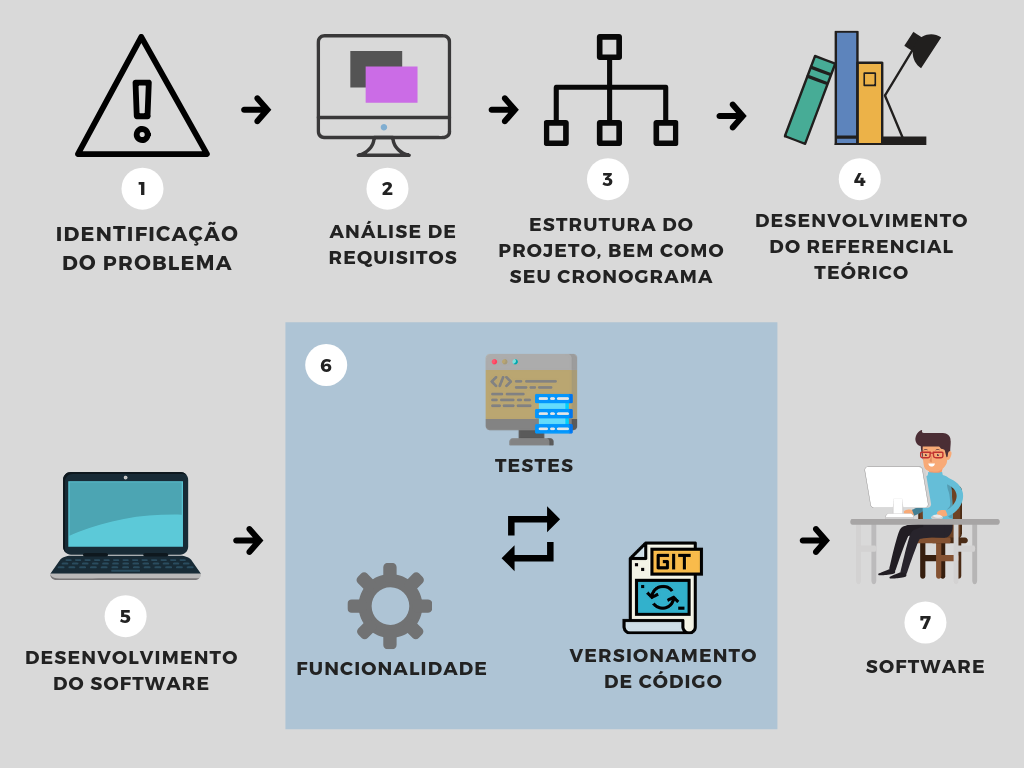
\includegraphics[scale=0.5]{5-Metodologia/metodologia-desenvolvimento-tcc.png}
	\end{center}
	\centering \legend{Fonte: Elaborada pelos autores.}
\end{figure}

%-- Fim Metodologia --%

%-- Inicio conteúdo desenvolvimento --%

\chapter{\textbf{DESENVOLVIMENTO}}
\label{desenvolvimento}

% Este capítulo tem por finalidade abordar todo o processo utilizado para o desenvolvimento desse projeto, relatando as principais ferramentas utilizadas e testes do algoritmo. O capítulo está dividido em seções, onde a \autoref{desenvolvimento-do-sistema} descreve o desenvolvimento do sistema, a seção \autoref{descricao-do-sistema} apresenta a descrição do sistema, etapas de funcionamento e seus riscos e restrições. A \autoref{requisitos} descreve os requisitos do sistema, a \autoref{explicacao-codigo} tem por objetivo descrever os códigos utilizados para a elaboração deste projeto e a \autoref{ambientes-de-teste} relata os ambientes de teste e os testes do software.

Este capítulo tem por finalidade abordar todo o processo utilizado para o desenvolvimento desse projeto, relatando as principais ferramentas utilizadas e testes do algoritmo. O capítulo está dividido em seções, onde a \autoref{descricao-do-sistema} apresenta a descrição do sistema, etapas de funcionamento e seus riscos e restrições. A \autoref{requisitos} descreve os requisitos do sistema, a \autoref{explicacao-codigo} tem por objetivo descrever os códigos utilizados para a elaboração deste projeto, a \autoref{testes_do_software} relata os testes e as análises do \textit{software} e a \autoref{ref_avaliacao_dos_resultados} descreve a avaliação dos resultados do \textit{software}.

%\section{\textbf{Desenvolvimento do sistema}}
\label{desenvolvimento-do-sistema}

COMO FOI FEITO

\section{\textbf{Descrição do sistema}}
\label{descricao-do-sistema}

% Antes de descrever qualquer coisa relacionada a ferramenta, é preciso entender que o \textit{software} passa por um aprendizado de máquina para aprender os padrões de características que são necessária para atender as necessidades do projeto, que é reconhecer um jogador em campo. O \textit{haar cascade} fica responsável por realizar a classificação da imagem para obter seus padrões de características. Basicamente, o \textit{haar cascade} é alimentado manualmente por imagens aleatórias de jogadores para montar um padrão de características e em seguida, esses padrões são treinados através do \textit{machine learning}. Isso deve ser feito para que seja possível obter um modelo de busca. Pode-se definir o modelo de busca como padrão de características de jogadores de futebol americano que será utilizado para realizar a busca.

O \textit{software} apresentado no decorrer deste projeto tem por objetivo reconhecer um jogador dentro de campo utilizando as técnicas de processamento de imagem para realizar a extração de todas as características importantes que estão presentes em uma imagem.

Antes de descrever qualquer coisa relacionada à ferramenta, é preciso entender que o \textit{software} passa por um aprendizado de máquina para extrair os padrões de características que são necessária para atender as necessidades do projeto, que é reconhecer um jogador em campo. Portanto, o sistema conta com a classificação de imagem para extrair as características relacionadas aos jogadores de futebol americano, conforme representado na \autoref{fig_ext_caracteristicas}.

\begin{figure}[h]
	\caption{\label{fig_ext_caracteristicas}Etapa de extração de características de uma imagem (A) e seu padrão de características (B).}
	\begin{center}
		\resizebox{.9\linewidth}{!}{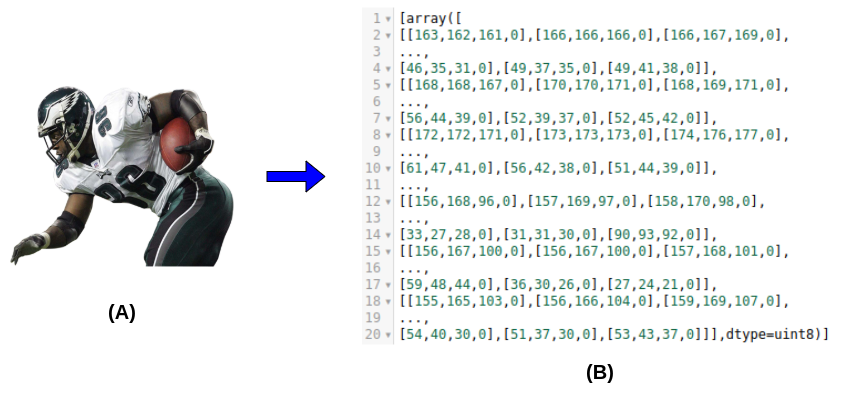
\includegraphics{6-Desenvolvimento-Projeto/imagens-desenvolvimento/conversao-de-imagem.png}}
	\end{center}
	\centering \legend{Fonte: Elaborada pelos autores.}
\end{figure}

% O \textit{haar cascade} fica responsável por realizar a classificação da imagem para obter seus padrões de características. Basicamente, o mesmo é alimentado manualmente por imagens aleatórias de jogadores de futebol americano para montar esse padrão de características. Sendo assim, pode-se definir o modelo de busca como o conjunto de padrões de características de jogadores de futebol americano que será utilizado para realizar a busca.

Quem fica responsável por realizar a classificação das imagens para obter seus padrões de características é o \textit{haar cascade}. Basicamente, o mesmo é alimentado manualmente por imagens aleatórias de jogadores de futebol americano para montar esse padrão de características. Sendo assim, pode-se definir o modelo de busca como um conjunto de padrões de características de jogadores de futebol americano que será utilizado para realizar a busca.

Em seguida, o \textit{software} passa pela etapa de \textit{machine learning} que ficará encarregada apenas de treinar o algoritmo utilizando os padrões de características. Ou seja, nessa etapa do processo, o sistema recebe como parâmetro os padrões de características extraídos na etapa anterior e analisa todos os seus pontos de interesse, montando o melhor modelo de busca.

Em seguida, o sistema recebe, através do dispositivo de captura de imagem, um vídeo em tempo real de uma partida de futebol americano.

O algoritmo realiza a análise de todos os \textit{frames}\footnote{\textit{Frames} por segundo é a taxa de atualização de imagens estáticas que formam uma cena animada dentro de um vídeo. A ilusão que nosso cérebro interpreta como movimento é feita através de vários quadros consecutivos em um curto período de tempo \cite{FRAMES2011}. \label{frames-por-segundo}} por segundo do vídeo para encontrar algo similar ao modelo de busca que foi treinado.

Caso ocorra a identificação de um jogador de futebol americano dentro do vídeo analisado, o algoritmo fica encarregado de realizar uma representação do mesmo. Essa representação será feita com um contorno verde ao redor do jogador.

\subsection{{Etapas de funcionamento do sistema}}

O funcionamento da ferramenta consiste em analisar uma imagem de um jogador objetivando adquirir todos os pontos de interesse da imagem, que servirá como parâmetro de busca para que o algoritmo seja mais eficiente quando o  mesmo for exposto a uma situação mais complexa como por exemplo, analisar um jogador com capacete.

A análise feita pelo algoritmo ocorre de forma minuciosa e utilizando técnicas de processamento de imagem. Sendo assim, após a extração de todos os pontos de interesse da imagem, o algoritmo monta um conjunto de sequências lógicas das taxas de \textit{pixels} existentes nesses pontos. Esta conversão pode ser demostrada de forma mais clara na \autoref{fig_conversao_img} da \autoref{descricao-do-sistema}.

Após a montagem do conjunto, o algoritmo utiliza um dispositivo de captura de imagem para realizar uma busca por similaridade, ou seja, o algoritmo buscará algo semelhante ao padrão montado na etapa anterior. Após a busca feita pelo \textit{software}, a detecção vai definir se existe ou não um jogador no ambiente que está sendo analisado. Se for constatado que existe um jogador e ele for igual ao modelo, a ferramenta vai apresentar o seu nome cadastrado. A \autoref{fig_fluxograma_proj} representa o fluxograma do \textit{software}.

\begin{figure}[h]
	\caption{\label{fig_fluxograma_proj}Fluxograma de funcionamento do sistema.}
	\begin{center}
		\resizebox{.9\linewidth}{!}{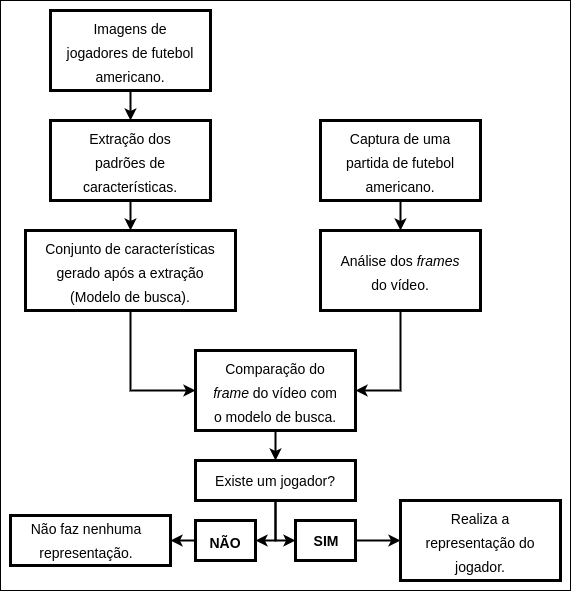
\includegraphics{6-Desenvolvimento-Projeto/imagens-desenvolvimento/fluxograma-projeto.png}}
	\end{center}
	\centering \legend{Fonte: Elaborada pelos autores.}
\end{figure}

Ao final do processo, será feito uma análise dos dados apresentados pela ferramenta. Através desses dados, pode-se obter o percentual de acertos e erros, analisando também os cenários de maior e menor eficiência.

\subsection{Restrições, riscos e exclusões do projeto}

As restrições do projeto podem ser definidas através de todos os fatores que limitam as funcionalidades do mesmo. Basicamente, são condições impostas para a elaboração do projeto que devem ser obrigatoriamente cumpridas pela equipe no decorrer do desenvolvimento do sistema. Com base nisso, as restrições deste projeto são:

\begin{itemize}
\raggedright \item Reconhecer pelo menos um jogador dentro de campo;
\raggedright \item Fazer a representação do jogador reconhecido.
% \item Somente o jogador que foi utilizado como modelo será representado. Caso algum outro jogador apareça na cena analisada, ele pode ser reconhecido como um jogador mais não terá nenhuma representação de reconhecimento, ou seja, o \textit{software} vai informar que o indivíduo é um jogador mas ele não o reconhecerá pelo nome.
\end{itemize}

Já a parte de riscos está relacionada a um evento ou situação incerta que pode afetar positivamente ou negativamente na execução do projeto. Descrevê-los é uma necessidade, para que saibamos identificar o momento certo que pode acontecer algum problema com relação ao software. Os riscos deste projeto são:

\begin{itemize}
\raggedright \item Se não houver uma boa iluminação, pode acontecer falhas no reconhecimento e até mesmo inutilizá-lo;
\raggedright \item A qualidade do sensor utilizado para capturar a imagem pode interferir no reconhecimento.
\end{itemize}

A exclusão consiste em todos os requisitos que estão explicitamente fora do projeto. Basicamente, é tudo aquilo que a equipe de desenvolvimento deixa claro que não será realizado ao longo do desenvolvimento do projeto. Sendo assim, segue a relação de requisitos que estão excluídos deste projeto:

\begin{itemize}
\raggedright \item Explicar matematicamente cada função executada;

\raggedright \item Reconhecer mais de um jogador dentro de campo;

\raggedright \item Solucionar algum possível problema identificado no processo de reconhecimento.
\end{itemize}

\section{\textbf{Requisitos}}
\label{requisitos}

\subsection{{Requisitos funcionais}}

Requisitos funcionais são responsáveis pelas funcionalidades, necessidades e características que definem um software, ou seja, eles definem o que o \textit{software} vai fazer, o seu comportamento. Os requisitos funcionais deste projeto são:

\begin{itemize}
\raggedright \item Realizar a classificação das imagens de jogadores de futebol americano.

\raggedright \item Gerar o \textit{haar cascade} com os pontos de interesses das imagens classificadas.

\raggedright \item Definir o modelo de busca a partir dos padrões de características dos jogadores de futebol americano.

\raggedright \item Realizar o treinamento do algoritmo com o modelo de busca definido.

\raggedright \item Capturar o vídeo através de um dispositivo (\textit{hardware}).

\raggedright \item Analisar cada \textit{frame} por segundo do vídeo.

\raggedright \item Identificar um jogador de futebol americano dentro de campo.

\raggedright \item Representar o jogador analisado.
\end{itemize}

\subsection{{Requisitos não-funcionais}}

Basicamente, requisitos não funcionais descrevem como o sistema fará alguma coisa. Sendo assim, os requisitos não funcionais estão relacionados ao desempenho do sistema, usabilidade, confiabilidade, restrições de projeto, manutenção e atributos da qualidade. São os seguintes:

\begin{itemize}
\raggedright \item O sistema deve ser implementado em \textit{phyton};

\raggedright \item O sistema necessita de dependências do \textit{phyton} para a sua execução;

\raggedright \item A biblioteca \textit{OpenCV} precisa estar instalada para a sua execução;

\raggedright \item O processamento da imagem será feito em \textit{hardware} próprio;

\raggedright \item O sistema requer grande processamento de \textit{hardware};

\raggedright \item Para a definição de um novo modelo, o sistema precisa passar por uma manutenção dos parâmetros de busca e, consequentemente, um novo treinamento da ferramenta;

\raggedright \item Para que o sistema possa ser executado, é necessário realizar comandos via terminal;

\raggedright \item O \textit{software} precisa de um dispositivo de captura de imagem como, por exemplo, uma \textit{Web Cam};

\raggedright \item O \textit{software} deve poder ser executado em \textit{Windows} e \textit{Linux}.

\end{itemize}

\section{\textbf{Explicando o código}}
\label{explicacao-codigo}
\definecolor{cinza}{rgb}{0.95,0.95,0.95}

Antes de explicar o código por trás do desenvolvimento deste projeto, é preciso informar que para executá-lo é necessário instalar a linguagem de programação \textit{Python} e suas dependências.

Para iniciar a codificação do algoritmo em \textit{Python}, é importante realizar a importações das bibliotecas necessárias para realizar o procedimento de reconhecimento. A biblioteca \textit{cv2} é a \textit{OpenCV}; a \textit{NumPy} fica responsável por realizar cálculos de vetores multidimensionais; a \textit{argparse} verifica e atribui os argumentos que são esperados; já a \textit{imutils} é responsável por converter a imagem em uma matriz.

\begin{minted}[linenos=true, mathescape, bgcolor=cinza]{python}

import cv2
import numpy as np
import argparse
import imutils

\end{minted}

Também é necessário importar os módulos da biblioteca \textit{imutils}.

\begin{minted}[linenos=true, mathescape, bgcolor=cinza]{python}

from __future__ import print_function
from imutils.object_detection import non_max_suppression
from imutils import paths

\end{minted}

Em seguida, o algoritmo deve ser programado para construir os argumentos necessários para iniciar o reconhecimento e analisar esses argumentos.

\begin{minted}[linenos=true, mathescape, bgcolor=cinza]{python}

ap = argparse.ArgumentParser()
ap.add_argument("-i", "--images", required=True,
    help="path to images directory")
args = vars(ap.parse_args())

\end{minted}

Agora é necessário iniciar o descritor \textit{HOG - Histogram of Oriented Gradients} (Histograma de Gradientes Orientados). Basicamente, o \textit{HOG} utiliza cálculos matemáticos extremamente complexos que serve para classificar dados da imagem e gerar um \textit{haar cascade} com suas configurações.

\begin{minted}[linenos=true, mathescape, bgcolor=cinza]{python}

hog = cv2.HOGDescriptor()
hog.setSVMDetector(cv2.HOGDescriptor_getDefaultPeopleDetector())

\end{minted}

Para o melhor desempenho do algoritmo, foi criado uma pasta local contendo todas as imagens necessárias para realizar a extração dos padrões de características dos jogadores de futebol americano. Sendo assim, o trecho de código a seguir serve para ler todas estas imagens que estão dentro da pasta \textit{images} localmente.

\begin{minted}[linenos=true, mathescape, bgcolor=cinza]{python}

imagePaths = list(paths.list_images(args["images"]))

\end{minted}

A partir desta etapa, o algoritmo vai executar uma estrutura de repetição para analisar todas as fotos alocadas na variável \textit{imagePaths} utilizada no trecho de código acima.

Sendo assim, o primeiro laço da estrutura de repetição fica responsável por carregar e redimensionar a imagem para reduzir o tempo de detecção. Em seguida, ele melhora a precisão da detecção da imagem para melhorar a extração de características.

\begin{minted}[linenos=true, mathescape, bgcolor=cinza]{python}

for imagePath in imagePaths:
	image = cv2.imread(imagePath)
	image = imutils.resize(image, width=min(400, image.shape[1]))
	orig = image.copy()

\end{minted}

Em seguida, ele tenta detectar se existe uma pessoa na imagem analisada.

\begin{minted}[linenos=true, mathescape, bgcolor=cinza]{python}

    (rects, weights) = hog.detectMultiScale(image, winStride=(4, 4),
        padding=(8, 8), scale=1.05)

\end{minted}

Apos isso, a segunda estrutura de repetição que está alocada dentro da primeira, fica responsável por delimita os locais onde contem os pontos de interesse dentro da imagem analisada, ou seja, o algoritmo seleciona as áreas de interesse que serão utilizadas como parâmetro de busca.

\begin{minted}[linenos=true, mathescape, bgcolor=cinza]{python}

    for (x, y, w, h) in rects:
	cv2.rectangle(orig, (x, y), (x + w, y + h), (0, 0, 255), 2)

\end{minted}

Em seguida, o \textit{software} realiza a técnica de supressão não máxima na imagem, ou seja, ele realiza a técnica de detecção de bordas para identificar os \textit{pixel} de maior intensidade e, em seguida, ele realiza a técnica de supressão para eliminar os \textit{pixels} que não possuem valores próximos aos da borda.

\begin{minted}[linenos=true, mathescape, bgcolor=cinza]{python}

    rects = np.array([[x, y, x + w, y + h] for (x, y, w, h) in rects])
	pick = non_max_suppression(rects, probs=None, overlapThresh=0.65)

\end{minted}

A terceira estrutura de repetição fica responsável por montar uma delimitação do indivíduo detectado na imagem analisada.

\begin{minted}[linenos=true, mathescape, bgcolor=cinza]{python}

    for (xA, yA, xB, yB) in pick:
		cv2.rectangle(image, (xA, yA), (xB, yB), (0, 255, 0), 2)

\end{minted}

Apos os procedimentos, o algoritmo fica responsável por desenhar as correspondências de informações contidas entre as imagens analisadas.

\begin{minted}[linenos=true, mathescape, bgcolor=cinza]{python}

    filename = imagePath[imagePath.rfind("/") + 1:]
	print("[INFO] {}: {} original boxes, {} after suppression".format
		(filename, len(rects), len(pick)))

\end{minted}

Por fim, o sistema mostra na tela a imagem analisada e os pontos de interesse que ele achou dentro da mesma. Na outra imagem, o \textit{software} mostra o que ele achou de semelhante após a análise.

\begin{minted}[linenos=true, mathescape, bgcolor=cinza]{python}

cv2.imshow("Before NMS", orig)
cv2.imshow("After NMS", image)
cv2.waitKey(0)

\end{minted}

A \autoref{fig_comparativo_img} descreve o que o sistema faz com a imagem e o seu resultado.

\begin{figure}[h]
	\caption{\label{fig_comparativo_img}A imagem (A) é a original, e as representações em vermelho são seus pontos de interesse. A imagem (B) é o resultado da detecção por bordas e seus pontos similares com a imagem (A).}
	\begin{center}
		\resizebox{.9\linewidth}{!}{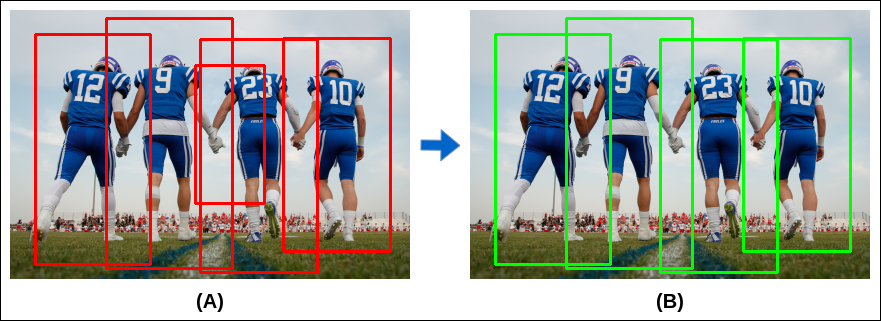
\includegraphics{6-Desenvolvimento-Projeto/imagens-desenvolvimento/comparativo_imagem.png}}
	\end{center}
	\centering \legend{Fonte: Elaborada pelos autores.}
\end{figure}

\subsection{{Testes do \textit{software}}}


\section{\textbf{Análise dos resultados}}

Para resumir os resultados obtidos nos testes de \textit{software}, foi feito uma tabela que tem por finalidade representar quais foram os ambientes de testes que o algoritmo foi submetido. Sendo assim, a \autoref{resultado_de_testes} mostra os resultados dos testes do algoritmo.

\begin{table}[h]
\centering
\caption{Resumo dos resultados dos testes}
\label{resultado_de_testes}
\begin{tabular}{l|l} 
\hline
\hline
\multicolumn{1}{l|}{Ambiente de Teste} & \multicolumn{1}{l}{Resultado}  \\ 
\hline
Partida de futebol americano & Positivo\\
Partida de futebol americano & Negativo\\
Jogador parado & Positivo\\
Jogador em movimento & Intermediário\\
Jogador de frente & Positivo\\
Jogador de costas & Positivo\\
\hline
\hline 
\end{tabular}
\end{table}

%-- Fim conteúdo desenvolvimento --%

\chapter{\textbf{CONSIDERAÇÕES FINAIS}}
\label{consideracoes_finais}

Escreva aqui as conclusões deste trabalho, lembrando que os objetivos geral e específicos devem ser citados e comentados,  ou seja, descreva como cada objetivo foi alcançado.

\section{\textbf{Propostas de novos estudos}}

% ----------------------------------------------------------

% ----------------------------------------------------------
% Finaliza a parte no bookmark do PDF
% para que se inicie o bookmark na raiz
% e adiciona espaço de parte no Sumário
% ----------------------------------------------------------
%\phantompart
% ----------------------------------------------------------
% ELEMENTOS PÓS-TEXTUAIS
% ----------------------------------------------------------
\postextual
% ----------------------------------------------------------

% ----------------------------------------------------------
% Referências bibliográficas
% ----------------------------------------------------------
%\bibliography{abntex2-modelo-references}
\bibliography{referencias}

% ----------------------------------------------------------
% Glossário
% ----------------------------------------------------------
%
% Consulte o manual da classe abntex2 para orientações sobre o glossário.
%
%\glossary

% ----------------------------------------------------------
% Apêndices
% ----------------------------------------------------------

% ---
% Inicia os apêndices
% ---
\begin{apendicesenv}
% Imprime uma página indicando o início dos apêndices
\partapendices
% ----------------------------------------------------------
\chapter{Primeiro Apêndice}

Testando
% ----------------------------------------------------------

\end{apendicesenv}
% ---


% ----------------------------------------------------------
% Anexos
% ----------------------------------------------------------

% ---
% Inicia os anexos
% ---
\begin{anexosenv}

% Imprime uma página indicando o início dos anexos
\partanexos

%-------------------------------------------------------------
\chapter{Primeiro Anexo.}

Testando
%-------------------------------------------------------------

\end{anexosenv}

%-------------------------------------------------------------
% INDICE REMISSIVO
%---------------------------------------------------------------------
\phantompart
\printindex
%---------------------------------------------------------------------

\end{document}
